% ******************************************************** %
%         TEMPLATE DE TESIS - TRAFFIC LIGHT DETECTION      %
% ******************************************************** %
% ******************************************************** %
%                                                          %
% ALGUNOS PAQUETES REQUERIDOS (EN UBUNTU):                 %
% ========================================
%                                                          %
% texlive-latex-base                                       %
% texlive-latex-recommended                                %
% texlive-fonts-recommended                                %
% texlive-latex-extra                                      %
% texlive-lang-spanish                                     %
% texlive-bibtex-extra                                     %
% ******************************************************** %


\documentclass[a4paper,12pt]{report}
\usepackage[spanish]{babel}
\usepackage[utf8]{inputenc}
\usepackage{charter}   % tipografia
\usepackage{graphicx}
\usepackage{subcaption} % para subfiguras en grids (2x2, 2x3, etc.)
\usepackage{tabularx}   % para tablas que se ajustan al ancho del texto
\graphicspath{{figures/}} % evita repetir "figures/" en cada includegraphics
\usepackage{paralist} %itemize inline
\usepackage{multirow} %tablas
\usepackage{float}
\usepackage{pgfplots}
\usepackage{algorithm}
\usepackage{algpseudocode}
\usepackage{verbatim}
\usepackage{forest,adjustbox}

% Para diagramas de pipelines
\usepackage{tikz}
\usetikzlibrary{shapes.geometric, arrows, arrows.meta, positioning, calc}

\usepackage{amsmath, amsthm, amssymb}

% \usepackage{underscore}  % Comentado - conflicto con caratula
\usepackage{caratula}
\usepackage{hyperref}

% Para links de colores
\hypersetup{
    colorlinks=true,
    linkcolor=blue,
    filecolor=magenta,
    urlcolor=cyan,
    citecolor=blue,
}

% ********************************************************* %
% ~~~~~~~~              Code snippets             ~~~~~~~~~ %
% ********************************************************* %

\usepackage{color} % para snippets de codigo coloreados
\usepackage{fancybox}  % para el sbox de los snippets de codigo

\definecolor{litegrey}{gray}{0.94}

\newenvironment{codesnippet}{%
	\begin{Sbox}\begin{minipage}{\textwidth}\sffamily\small}%
	{\end{minipage}\end{Sbox}%
		\begin{center}%
		\vspace{-0.4cm}\colorbox{litegrey}{\TheSbox}\end{center}\vspace{0.3cm}}

% Para código Python con syntax highlighting
% \usepackage{minted}  % Comentado temporalmente - requiere -shell-escape

% ********************************************************* %
% ~~~~~~~~         Formato de las páginas         ~~~~~~~~~ %
% ********************************************************* %

\usepackage{fancyhdr}
\pagestyle{fancy}

\renewcommand{\chaptermark}[1]{\markboth{\chaptername\ \thechapter.\ #1}{}}
\renewcommand{\sectionmark}[1]{\markright{\thesection\ #1}}

\fancyhf{}

\fancyhead[L]{\leftmark}
\fancyfoot[L]{\small{Ciro Juan Brignolo}}
\fancyfoot[R]{\thepage}
\renewcommand{\headrulewidth}{0.5pt}
\renewcommand{\footrulewidth}{0.5pt}
\setlength{\hoffset}{-0.8in}
\setlength{\textwidth}{16cm}
\setlength{\headsep}{0.5cm}
\setlength{\textheight}{25cm}
\setlength{\voffset}{-0.7in}
\setlength{\headwidth}{\textwidth}
\setlength{\headheight}{13.1pt}

\renewcommand{\baselinestretch}{1.3}  % line spacing (1.3 para tesis)

% ******************************************************** %

\usepackage{titlesec}

\setcounter{secnumdepth}{4}
\setcounter{tocdepth}{4}

\titleformat{\paragraph}
{\normalfont\normalsize\bfseries}{\theparagraph}{1em}{}
\titlespacing*{\paragraph}
{0pt}{3.25ex plus 1ex minus .2ex}{1.5ex plus .2ex}
\providecommand{\norm}[1]{\lVert#1\rVert}

% ******************************************************** %
% ~~~~~~~~         Información de la tesis        ~~~~~~~~~ %
% ******************************************************** %

\begin{document}

\thispagestyle{empty}
\materia{Licenciatura en Ciencias de la Computaci\'on}
\submateria{Trabajo Final de Licenciatura}
\titulo{Aislamiento de un M\'odulo de Detecci\'on de Sem\'aforos para Hacer Testing}
\subtitulo{Un Enfoque Basado en el An\'alisis y Modularizaci\'on del Sistema Apollo}
\fecha{2025}
\integrante{Ciro Juan Brignolo}{707/16}{cirob100@gmail.com}

\maketitle
\newpage

% ******************************************************** %
% ~~~~~~~~              Resumen/Abstract          ~~~~~~~~~ %
% ******************************************************** %

\thispagestyle{empty}
\chapter*{Resumen}
\addcontentsline{toc}{chapter}{Resumen}

Los sistemas de conducción autónoma son infraestructuras de software complejas que integran múltiples componentes de \textit{machine learning}. El testing exhaustivo de estos sistemas es fundamental para garantizar su confiabilidad y seguridad, pero la complejidad y el acoplamiento del sistema completo dificultan el diseño de tests específicos y controlados sobre componentes individuales.

Este trabajo presenta una metodología de testing basada en el \textbf{aislamiento} de un subsistema crítico: la idea es modularizar la lógica funcional de un componente sacándola del entorno acoplado del sistema original, para poder ejercitarla en condiciones controladas. Como caso de estudio se eligió el módulo de detección de semáforos (Traffic Light Recognition, TLR) del sistema Apollo de Baidu. Se analizó el código original para extraer su estructura, parámetros y reglas de decisión, y se construyó un módulo aislado funcionalmente equivalente que se ejecuta sin la infraestructura del vehículo (CyberRT, Bazel, Docker, HD-Map dinámico). La reimplementación en Python aparece solo como medio práctico para concretar ese aislamiento: el objetivo no es un sistema mejor, sino una versión del módulo sobre la que tengamos control total.

El proceso incluyó: (1) un primer intento fallido de recortar el código original C++ del sistema completo, descartado por el costo desproporcionado de su infraestructura; (2) un análisis iterativo del código fuente para extraer especificaciones funcionales no documentadas; (3) la construcción del módulo aislado a partir de ese análisis; (4) la definición de un conjunto de supuestos de equivalencia funcional con el módulo original; y (5) el diseño de tests exploratorios basados en el conocimiento interno adquirido durante el aislamiento.

Los resultados muestran la viabilidad del enfoque: el módulo aislado permitió diseñar tests difícilmente realizables sobre el sistema completo, y el proceso reveló decisiones de diseño y parámetros no documentados oficialmente (ponderación 70/30 del algoritmo húngaro, funcionalidad de \textit{semantic ID} diseñada pero hardcodeada a 0 en el código, ventana temporal de 1.5\,s del \textit{tracking} con histéresis, restricción del \textit{blink detection} al color verde con umbral de 0.55\,s).

\textbf{Palabras clave:} testing de software, sistemas de conducción autónoma, aislamiento de subsistemas, modularización, oracle-based testing, detección de semáforos, machine learning, Apollo, PyTorch

\newpage

% ******************************************************** %
% ~~~~~~~~         Tabla de contenidos           ~~~~~~~~~ %
% ******************************************************** %

\thispagestyle{empty}
\tableofcontents
\newpage

% ******************************************************** %
% ~~~~~~~~         Lista de figuras              ~~~~~~~~~ %
% ******************************************************** %

\listoffigures
\newpage

% ******************************************************** %
% ~~~~~~~~              CAPÍTULOS                ~~~~~~~~~ %
% ******************************************************** %

\chapter{Introducción}
\label{cap:introduccion}

\section{Motivación}

Los sistemas de conducción autónoma integran múltiples componentes de software que deben operar de manera coordinada para garantizar la seguridad. Entre estos componentes, los módulos de percepción basados en machine learning son particularmente difíciles de testear: no tienen especificaciones formales completas, su comportamiento se aprende de datos, y pueden fallar de formas sutiles e inesperadas.

El testing de estos sistemas presenta un desafío fundamental: ¿cómo diseñar tests efectivos para un componente cuyo comportamiento correcto no está formalmente especificado? Este trabajo propone que la respuesta está en el \textbf{conocimiento interno del sistema}. Si comprendemos profundamente cómo funciona un componente ---sus parámetros, sus reglas de decisión, sus casos límite--- podemos diseñar tests que exploten ese conocimiento para encontrar comportamientos anómalos.

Sin embargo, los sistemas de conducción autónoma como Apollo de Baidu son extremadamente complejos: millones de líneas de código, decenas de dependencias, configuraciones específicas de hardware. Esta complejidad dificulta tanto la comprensión del sistema como el diseño de tests controlados.

\section{Propuesta}

Este trabajo propone una metodología basada en \textbf{recortar y reimplementar} un subsistema crítico para poder comprenderlo profundamente y testearlo de forma controlada.

La idea central es:

\begin{enumerate}
    \item \textbf{Seleccionar un subsistema funcionalmente relevante} del sistema completo
    \item \textbf{Reimplementarlo} de forma fiel pero simplificada, eliminando complejidad accidental (dependencias, configuraciones)
    \item \textbf{Usar el conocimiento adquirido} durante la reimplementación para diseñar tests específicos
    \item \textbf{Buscar adversarios}: casos de test que revelen debilidades del sistema mediante análisis de caja blanca
\end{enumerate}

\subsection{¿Por qué reimplementar?}

El objetivo no es crear un sistema mejor, sino obtener un \textbf{subsistema equivalente sobre el cual tengamos control total}. Esto permite:

\begin{itemize}
    \item \textbf{Comprensión profunda:} Reimplementar fuerza a entender cada detalle del sistema original
    \item \textbf{Simplicidad:} Eliminar dependencias innecesarias facilita la experimentación
    \item \textbf{Instrumentación:} Agregar logging, visualizaciones, modificaciones para testing
    \item \textbf{Fidelidad:} Si la reimplementación es equivalente, los hallazgos aplican al sistema original
\end{itemize}

\subsection{¿Por qué buscar adversarios mediante caja blanca?}

La hipótesis central de este trabajo es que si tenemos acceso al código y comprendemos la lógica interna de un sistema, podemos diseñar tests más efectivos que con testing de caja negra. Específicamente:

\begin{itemize}
    \item Podemos identificar \textbf{parámetros críticos} (thresholds, pesos) y testear cerca de sus límites
    \item Podemos encontrar \textbf{reglas de negocio} y diseñar inputs que las violen
    \item Podemos descubrir \textbf{funcionalidades no implementadas} que podrían causar problemas
    \item Podemos entender \textbf{modos de falla} analizando la lógica de clasificación
\end{itemize}

\section{Caso de Estudio}

Como caso de estudio, seleccionamos el módulo de detección de semáforos (Traffic Light Recognition - TLR) del sistema Apollo de Baidu \cite{apollo_auto}.

\subsection{Criterios de Selección}

\begin{enumerate}
    \item \textbf{Criticidad:} La detección de semáforos es un componente de seguridad crítico

    \item \textbf{Simplicidad relativa:} Solo requiere cámaras (no LiDAR), tiene un espacio de salida limitado (rojo, amarillo, verde, apagado)

    \item \textbf{Interfaces claras:} Input (imagen + regiones de interés) → Output (detecciones + estados)

    \item \textbf{Código disponible:} Apollo es open source, permitiendo análisis completo
\end{enumerate}

\subsection{Apollo}

Apollo es una plataforma de código abierto para vehículos autónomos desarrollada por Baidu \cite{apollo_auto}. El módulo TLR es responsable de detectar semáforos en imágenes de cámara, reconocer su estado actual, y mantener tracking temporal de los semáforos a lo largo del tiempo.

\section{Contribuciones}

Las contribuciones de este trabajo son:

\begin{enumerate}
    \item \textbf{Metodología de recorte y reimplementación:} Demostración de que reimplementar un subsistema es más viable que intentar recortarlo del sistema complejo original

    \item \textbf{Análisis del sistema Apollo:} Documentación de decisiones de diseño no documentadas, parámetros extraídos, y hallazgos sobre el sistema

    \item \textbf{Criterios de conformidad:} Definición de qué significa que el recorte sea ``equivalente'' al original

    \item \textbf{Proceso de testing basado en conocimiento interno:} Diseño de tests específicos aprovechando la comprensión profunda del sistema

    \item \textbf{Validación de la hipótesis:} Demostración de que el análisis de caja blanca permite encontrar adversarios (caso del test de transición verde→amarillo)
\end{enumerate}

\section{Estructura del Trabajo}

Este trabajo se organiza de la siguiente manera:

\begin{itemize}
    \item \textbf{Capítulo \ref{cap:marco_teorico} - Marco Teórico:} Conceptos necesarios para comprender el trabajo, incluyendo todo lo conocido previamente sobre Apollo

    \item \textbf{Capítulo \ref{cap:analisis_apollo} - Análisis del Sistema:} El proceso de análisis de Apollo, las preguntas que guiaron el trabajo, y los hallazgos que justificaron las decisiones de recorte

    \item \textbf{Capítulo \ref{cap:reimplementacion} - Reimplementación:} Objetivos del recorte, alcance funcional, criterios de conformidad, y el proceso de reimplementación incluyendo la validación de equivalencia

    \item \textbf{Capítulo \ref{cap:diseno_tests} - Testing:} Diseño de tests basados en conocimiento interno del sistema, con foco en el test de transición verde→amarillo

    \item \textbf{Capítulo \ref{cap:resultados} - Resultados:} Hallazgos del proceso de testing y análisis

    \item \textbf{Capítulo \ref{cap:conclusiones} - Conclusiones:} Lecciones aprendidas, limitaciones, y trabajo futuro
\end{itemize}
\chapter{Marco Teórico}
\label{cap:marco_teorico}

Este capítulo presenta los conceptos necesarios para comprender el trabajo y una presentación mínima del sistema Apollo. El detalle del módulo TLR ---sus etapas, parámetros y reglas--- se introduce de forma narrativa en el Capítulo~\ref{cap:analisis_apollo}, donde forma parte del proceso de análisis.

\section{Conceptos de Testing}

\subsection{Oracle-Based Testing}

Un \textit{test oracle} es un mecanismo para determinar si un test ha pasado o fallado \cite{barr2015oracle}. En este trabajo, el sistema Apollo original actúa como oráculo: el módulo aislado se considera correcto si produce los mismos resultados que Apollo para las mismas entradas, dadas las mismas condiciones.

\textbf{Limitación:} este enfoque asume que Apollo es correcto. Si Apollo tiene bugs, el módulo aislado los replicará. La validez del oráculo es relativa: lo que se está validando es la \textit{equivalencia} con el sistema de referencia, no la corrección absoluta.

\subsection{Testing de Caja Blanca vs. Caja Negra}

\textbf{Caja negra:} diseñar tests basándose únicamente en la especificación de entrada/salida, sin conocer la implementación interna.

\textbf{Caja blanca:} diseñar tests aprovechando el conocimiento de la implementación interna: parámetros, \textit{thresholds}, reglas de decisión, casos límite, ramas del flujo de control.

Este trabajo argumenta que para sistemas de \textit{machine learning} sin especificación formal, el testing de caja blanca es particularmente efectivo: permite diseñar tests que apuntan a comportamientos específicos de la implementación, que el testing de caja negra difícilmente encontraría de manera sistemática. El aislamiento del módulo es lo que vuelve viable este enfoque, al ofrecer un objeto manipulable cuyas tripas son accesibles.

\subsection{Testing Exploratorio}

El testing exploratorio consiste en diseñar y ejecutar tests de forma simultánea, ajustando la estrategia con base en el conocimiento adquirido durante el proceso. A diferencia del testing planificado, los tests se diseñan iterativamente a medida que se comprende mejor el sistema. Este enfoque es particularmente útil para sistemas de \textit{machine learning} donde el comportamiento correcto no está formalmente especificado y donde cada ejecución revela nuevas hipótesis a probar.

\section{Reverse Engineering de Software}

El \textit{reverse engineering} es el proceso de analizar un sistema para extraer sus especificaciones a partir del código fuente \cite{chikofsky1990reverse}.

En este trabajo se aplicaron dos técnicas:

\textbf{Análisis estático:} examinar el código sin ejecutarlo para extraer parámetros, estructuras de datos y lógica de decisión. Es la técnica predominante en el análisis del módulo TLR, ya que las dependencias de Apollo dificultan la ejecución del código original (ver Capítulo~\ref{cap:reimplementacion}).

\textbf{Análisis dinámico:} ejecutar el sistema con \textit{inputs} conocidos para observar y validar el comportamiento. En este trabajo, el análisis dinámico se realizó sobre el módulo \textit{aislado}, no sobre el original, una vez que la versión aislada fue construida.

\section{Componentes Técnicos}

\subsection{Intersection over Union (IoU)}

Métrica para medir solapamiento entre \textit{bounding boxes}:

\begin{equation}
IoU(A, B) = \frac{|A \cap B|}{|A \cup B|}
\end{equation}

Se usa en \textit{Non-Maximum Suppression} (NMS) para eliminar detecciones duplicadas que se solapan por encima de un umbral.

\subsection{Algoritmo Húngaro}
\label{sec:algoritmo_hungaro}

\subsubsection{El problema de asignación}

El algoritmo húngaro \cite{kuhn1955hungarian} resuelve el \textbf{problema de asignación}: dado un conjunto de $n$ ``agentes'' y un conjunto de $n$ ``tareas'', y una matriz de costos $C \in \mathbb{R}^{n\times n}$ donde $C_{ij}$ es el costo (o beneficio) de asignarle la tarea $j$ al agente $i$, se busca una asignación uno-a-uno que minimice (o maximice) el costo total. Formalmente, se busca una permutación $\sigma$ de $\{1,\dots,n\}$ que minimice
\[
\sum_{i=1}^{n} C_{i,\sigma(i)}.
\]
La asignación es \textit{biyectiva}: cada agente recibe exactamente una tarea, y cada tarea es ejecutada por exactamente un agente. Para conjuntos de tamaños distintos $m\neq n$, la matriz se rellena con filas o columnas \textit{dummy} de costo neutro hasta hacerla cuadrada; las asignaciones contra \textit{dummies} se descartan al final.

\subsubsection{Origen y nomenclatura}

El método fue formulado por Harold W.\ Kuhn en 1955 \cite{kuhn1955hungarian}, basándose en trabajos previos de los matemáticos húngaros Dénes Kőnig y Jenő Egerváry, de donde proviene el nombre. En 1957, James Munkres demostró que el algoritmo termina en tiempo polinomial; por eso también se lo conoce como \textbf{algoritmo de Kuhn-Munkres} o, en implementaciones de ingeniería, simplemente como ``Munkres''. El archivo \texttt{hungarian\_optimizer.h} del código de Apollo y el archivo \texttt{hungarian\_optimizer.py} del módulo aislado se refieren a esta misma idea con los dos nombres usados de manera intercambiable.

\subsubsection{Cómo funciona}

La intuición detrás del algoritmo es que el problema no cambia si a una fila o columna entera de la matriz de costos se le suma o resta una constante: la asignación óptima sigue siendo la misma, aunque el valor total cambie. El algoritmo explota esta invariancia para transformar la matriz original en otra equivalente que tenga \textit{ceros suficientes} como para describir la solución óptima.

El procedimiento clásico tiene seis pasos, repetidos hasta que se alcanza una asignación válida:

\begin{enumerate}
    \item \textbf{Reducción de filas:} a cada fila se le resta su elemento mínimo. Después de este paso, cada fila tiene al menos un cero.
    \item \textbf{Reducción de columnas:} análogamente, a cada columna se le resta su mínimo.
    \item \textbf{Cobertura mínima:} se cubre el conjunto de ceros de la matriz con el menor número posible de líneas (filas o columnas enteras). Si ese número es igual a $n$, los ceros ya son suficientes para describir una asignación óptima y el algoritmo termina.
    \item \textbf{Ajuste de la matriz:} si la cobertura usó menos de $n$ líneas, se identifica el menor elemento no cubierto y se resta a todos los elementos no cubiertos, sumándoselo a los doblemente cubiertos. Esto preserva la equivalencia con la matriz original y crea nuevos ceros.
    \item \textbf{Búsqueda de \textit{augmenting paths}:} a partir del estado actual, se busca un camino alternante de ceros que permita mejorar la asignación parcial.
    \item \textbf{Extracción de la asignación:} cuando los ceros cubren la matriz con $n$ líneas, se eligen $n$ ceros independientes (uno por fila y por columna) y esos son los pares $(i, \sigma(i))$ de la asignación óptima.
\end{enumerate}

La complejidad del algoritmo es $O(n^3)$ en su versión clásica, lo cual es totalmente manejable para los tamaños típicos del problema de detección de semáforos (raramente más de 5 o 6 semáforos visibles a la vez).

\subsubsection{Maximización vs.\ minimización}

El algoritmo está formulado para \textit{minimizar} el costo total, pero el problema en detección de semáforos es de \textit{maximización} (queremos la asignación que maximice la suma de \textit{scores}). La conversión es trivial: si $S$ es la matriz de \textit{scores} y $S_{\max}$ es su máximo, se ejecuta el algoritmo sobre la matriz $C = S_{\max} - S$. La permutación óptima resultante es la misma, y el valor maximizado se reconstruye con $\sum S_{i,\sigma(i)} = n\cdot S_{\max} - \sum C_{i,\sigma(i)}$.

\subsubsection{Uso en el módulo TLR}

En el contexto de detección de semáforos, el algoritmo se usa para asignar las $N$ detecciones de la red neuronal a las $M$ regiones de interés conocidas (\textit{projection boxes}). El \textit{score} a maximizar combina proximidad espacial y confianza de la detección, con una ponderación específica que se detalla en el Capítulo~\ref{cap:funcionamiento_tlr}. El resultado es una correspondencia biyectiva entre detecciones y \textit{projection boxes} que el resto del pipeline trata como ``esta detección corresponde a este semáforo del HD-Map''.

\subsection{Conversión Caffe a PyTorch}

Apollo utiliza modelos en formato Caffe (\textit{framework} legacy). La construcción de un módulo aislado en Python requiere:

\begin{enumerate}
    \item Parsear archivos \texttt{.prototxt} (definición de arquitectura).
    \item Mapear capas Caffe a equivalentes en PyTorch.
    \item Cargar pesos desde archivos \texttt{.caffemodel}.
    \item Validar equivalencia numérica de \textit{outputs} capa por capa.
\end{enumerate}

Esta conversión no introduce cambios funcionales: la arquitectura, los pesos y la aritmética son los mismos; sólo cambia el \textit{runtime} sobre el que se evalúa la red.

\section{El Sistema Apollo: Presentación}

\subsection{Visión General}

Apollo es una plataforma \textit{open source} para vehículos autónomos desarrollada por Baidu \cite{apollo_auto}. Integra módulos para:

\begin{itemize}
    \item \textbf{Percepción:} detección de obstáculos, semáforos, carriles.
    \item \textbf{Predicción:} predicción de trayectorias de otros vehículos.
    \item \textbf{Planificación:} planificación de ruta y maniobras.
    \item \textbf{Control:} control de actuadores del vehículo.
\end{itemize}

El sistema está construido sobre infraestructura propia: el \textit{framework} de mensajería \textbf{CyberRT}, el sistema de \textit{build} \textbf{Bazel}, contenedores Docker para \textit{deployment}, y el \textit{framework} de \textit{deep learning} Caffe para los modelos. Esta infraestructura es transversal a casi todos los módulos: un cambio o una ejecución parcial del sistema rara vez puede hacerse sin tocarla.

\subsection{Paper de FSE 2020}

El paper ``A First Look at the Integration of Machine Learning Models in Complex Autonomous Driving Systems'' \cite{peng2020first} analiza cómo se integran los modelos de \textit{machine learning} en Apollo e identifica:

\begin{itemize}
    \item \textbf{Acoplamiento estrecho:} los componentes están fuertemente integrados.
    \item \textbf{Dependencias de hardware:} muchos componentes requieren GPUs específicas.
    \item \textbf{Complejidad de configuración:} el despliegue requiere configuraciones extensas.
\end{itemize}

Este paper motivó la idea central del trabajo: si extraer y ejercitar un subsistema aislado puede facilitar su testing, vale la pena explorar la metodología sobre un módulo concreto.

\subsection{El Módulo TLR como Caso de Estudio}

El módulo TLR (\textit{Traffic Light Recognition}) de Apollo es responsable de detectar semáforos en imágenes de cámara, reconocer su estado actual y mantener \textit{tracking} temporal. A nivel macro, su pipeline incluye preprocesamiento de regiones de interés, una red de detección, una red de reconocimiento de color y una etapa de \textit{tracking} temporal con reglas de seguridad. El Capítulo~\ref{cap:analisis_apollo} presenta el módulo a través del análisis que se hizo de él, y el Capítulo~\ref{cap:funcionamiento_tlr} profundiza en el detalle técnico de cada etapa.

\subsection{Lo No Documentado}

Aunque la documentación oficial de Apollo describe el pipeline a alto nivel, varios aspectos críticos \textbf{no están documentados}:

\begin{itemize}
    \item Valores específicos de parámetros (\textit{thresholds}, pesos, sigmas).
    \item Reglas de seguridad del \textit{tracking} temporal.
    \item Lógica de decisión en casos ambiguos.
    \item Justificación de decisiones de diseño.
    \item Funcionalidades diseñadas pero no efectivamente implementadas.
\end{itemize}

Estos aspectos solo se pueden descubrir mediante análisis del código fuente, lo cual constituye una parte central del trabajo de esta tesis.

\section{Resumen}

Este capítulo presentó:

\begin{itemize}
    \item Conceptos de testing relevantes: \textit{oracle-based testing}, caja blanca vs.\ caja negra, testing exploratorio.
    \item Técnicas de \textit{reverse engineering}: análisis estático y análisis dinámico.
    \item Componentes técnicos: IoU, algoritmo húngaro, conversión Caffe→PyTorch.
    \item Una presentación mínima del sistema Apollo, suficiente para situar el caso de estudio.
\end{itemize}

El siguiente capítulo aborda el análisis del módulo TLR: las preguntas que guiaron el trabajo, cómo está construido el módulo dentro de Apollo a nivel narrativo, qué hallazgos del código fuente fueron determinantes, y qué decisiones de aislamiento se desprenden de ese análisis. El Capítulo~\ref{cap:funcionamiento_tlr} retoma luego el detalle técnico de cada una de sus etapas, y el Capítulo~\ref{cap:reimplementacion} describe la construcción del módulo aislado.
\chapter{Análisis del Módulo TLR}
\label{cap:analisis_apollo}

Este capítulo describe el proceso de análisis del módulo de detección de semáforos (\textit{Traffic Light Recognition}, TLR) de Apollo. El objetivo del análisis no fue documentar el módulo por sí mismo, sino reunir el conocimiento necesario para poder aislarlo: entender qué hace, cuáles son sus límites, qué necesita del resto del sistema y qué simplificaciones serían aceptables.

El capítulo sigue ese orden. Primero plantea las preguntas que guiaron el análisis. Después responde a alto nivel cómo está organizado el módulo dentro de Apollo y qué hacen sus etapas, acompañado de un diagrama de bloques y un diagrama de secuencia con \textit{input}/\textit{output}. Luego presenta los hallazgos del código fuente que resultaron determinantes para el aislamiento. Y cierra con las decisiones de aislamiento que se desprenden de todo lo anterior. El detalle técnico de cómo funciona cada etapa internamente se posterga al Capítulo~\ref{cap:funcionamiento_tlr}, donde tiene espacio propio.

\section{Preguntas que Guiaron el Análisis}
\label{sec:preguntas_analisis}

El análisis estuvo orientado por cuatro preguntas. Cada una apunta a una decisión concreta de aislamiento.

\begin{enumerate}
    \item \textbf{¿Cuál es el alcance funcional del módulo TLR?} \\
    ¿Qué hace exactamente? ¿Cuáles son sus entradas y salidas? ¿De qué otros módulos depende para funcionar?

    \item \textbf{¿Qué partes del código son esenciales y cuáles son accesorias?} \\
    ¿Qué es lógica \textit{core} del TLR (decisiones, parámetros, modelos) y qué es infraestructura del entorno Apollo (CyberRT, Bazel, integración con otros módulos)? El aislamiento depende de poder hacer esta distinción.

    \item \textbf{¿Qué parámetros y reglas de decisión utiliza el sistema?} \\
    ¿Cuáles son los \textit{thresholds}, pesos y reglas de negocio que determinan el comportamiento observable? Estos son los que el módulo aislado debe reproducir.

    \item \textbf{¿Qué simplificaciones podemos hacer sin afectar la lógica \textit{core}?} \\
    ¿Qué dependencias podemos eliminar manteniendo equivalencia funcional? ¿Qué se puede reemplazar por una interfaz más simple sin perder la semántica del módulo?
\end{enumerate}

Las dos primeras preguntas delimitan qué entra al módulo aislado y qué queda afuera. La tercera define qué se debe preservar. La cuarta habilita la modularización: identifica qué piezas del entorno original pueden ser reemplazadas por equivalentes más simples sin que el comportamiento del módulo cambie.

\section{El Módulo TLR dentro de Apollo}

\subsection{Ubicación en el Código}

El TLR no es un único componente monolítico, sino un conjunto de cuatro subcomponentes que viven en \texttt{modules/perception/} del repositorio de Apollo:

\begin{verbatim}
modules/perception/
|-- traffic_light_region_proposal/  # Generacion de ROIs desde HD-Map
|-- traffic_light_detection/        # Deteccion de semaforos en imagen
|-- traffic_light_recognition/      # Clasificacion de color
`-- traffic_light_tracking/         # Tracking temporal y reglas
\end{verbatim}

Cada subcomponente es un \textit{component} en el sentido de Apollo: tiene sus propios archivos de configuración (\texttt{.pb.txt}, \texttt{.proto}), sus reglas de \textit{build} para Bazel (\texttt{BUILD}), su descripción de despliegue (\texttt{cyberfile.xml}, \texttt{.dag}, \texttt{.launch}) y su código fuente. Los cuatro componentes se ejecutan en cadena dentro del proceso de percepción del vehículo, comunicándose a través del \textit{framework} de mensajería CyberRT.

\subsection{Infraestructura de la que Depende}

Para que los cuatro componentes funcionen, Apollo necesita además infraestructura que es transversal al sistema completo:

\begin{itemize}
    \item \textbf{CyberRT:} \textit{framework} de mensajería propio que orquesta la comunicación entre componentes a través de \textit{channels}. Sin CyberRT no hay forma estándar de pasar un \textit{frame} de la cámara al componente de detección.
    \item \textbf{Map module:} acceso al HD-Map. El componente de \textit{region proposal} consulta el HD-Map en tiempo real para saber dónde hay semáforos cerca del vehículo.
    \item \textbf{Perception common:} utilidades compartidas con el resto del módulo de percepción: \textit{inference engines}, transformaciones de coordenadas, primitivas geométricas.
    \item \textbf{Modules common:} utilidades transversales del sistema (\textit{math}, \textit{configs}, \textit{logging}).
    \item \textbf{Calibración de cámara:} parámetros intrínsecos y extrínsecos del vehículo que se usan para proyectar coordenadas 3D del mundo a píxeles de imagen.
    \item \textbf{Caffe (vía libtorch):} \textit{framework} de \textit{deep learning} sobre el que corren los cuatro modelos del TLR. Requiere CUDA y una GPU NVIDIA específica.
\end{itemize}

El TLR no puede ejecutarse sin esta infraestructura; cualquier estrategia de aislamiento tiene que decidir qué se hace con ella.

\section{Cómo Funciona el Módulo: Vista a Alto Nivel}

\subsection{Las Cinco Etapas}

El pipeline del TLR procesa cada \textit{frame} de la cámara en cinco etapas secuenciales:

\begin{enumerate}
    \item \textbf{Preprocesamiento (\textit{Region Proposal}).} A partir de la posición del vehículo y el HD-Map, calcula qué semáforos físicos deberían aparecer en la imagen y proyecta sus coordenadas 3D del mundo a regiones rectangulares 2D en la imagen (\textit{projection boxes}). También decide qué cámara usar cuando hay varias disponibles. Cada semáforo identificado mantiene un \textit{signal\_id} persistente proveniente del HD-Map.

    \item \textbf{Detección.} Para cada \textit{projection box}, recorta una región expandida de la imagen y la pasa por una red convolucional (estilo \textit{Faster R-CNN}) que devuelve detecciones de semáforos con un \textit{bounding box} y un tipo (vertical, horizontal, \textit{quad}). Las detecciones no llevan identidad: son simplemente recuadros en la imagen.

    \item \textbf{Asignación.} Vincula cada detección de la red con la \textit{projection box} que mejor le corresponde. Usa el algoritmo húngaro sobre una matriz de costos que combina proximidad espacial y confianza de detección. Su salida son pares ($i$, $j$) que dicen ``la \textit{projection box} $i$ corresponde a la detección $j$'', y por lo tanto a un \textit{signal\_id} concreto.

    \item \textbf{Reconocimiento.} Para cada semáforo detectado, recorta el \textit{bounding box} de la detección y lo pasa por una de tres redes convolucionales especializadas (una por orientación: vertical, horizontal, \textit{quad}). La red devuelve probabilidades para cuatro estados: apagado (\textit{black}), rojo, amarillo y verde.

    \item \textbf{Tracking.} Mantiene un historial por \textit{signal\_id} a través de los \textit{frames}. Aplica reglas de consistencia temporal y de seguridad: transiciones de color inválidas se corrigen, detecciones aisladas de ``apagado'' no destruyen el color anterior, y se detecta parpadeo en verde con una ventana temporal específica.
\end{enumerate}

La Figura~\ref{fig:pipeline_alto_nivel} muestra las cinco etapas como bloques. La Figura~\ref{fig:diagrama_secuencia} las muestra como un diagrama de secuencia donde cada flecha indica el \textit{input}/\textit{output} que pasa de una etapa a la siguiente.

\subsection{Diagrama de Bloques}

\begin{figure}[H]
\centering
\begin{tikzpicture}[
    node distance=0.55cm,
    block/.style={rectangle, draw, rounded corners, minimum width=8.5cm, minimum height=0.9cm, align=center, font=\small},
    io/.style={rectangle, draw, dashed, rounded corners, minimum width=8.5cm, minimum height=0.8cm, align=center, font=\small\itshape},
    arrow/.style={-{Latex[length=2.5mm]}, thick}
]
    \node[io] (in) {Frame de cámara + Pose del vehículo + HD-Map};
    \node[block, below=of in] (preproc) {1. Preprocesamiento (\textit{Region Proposal})};
    \node[block, below=of preproc] (det) {2. Detección};
    \node[block, below=of det] (asg) {3. Asignación (algoritmo húngaro)};
    \node[block, below=of asg] (rec) {4. Reconocimiento};
    \node[block, below=of rec] (trk) {5. Tracking};
    \node[io, below=of trk] (out) {Estados de semáforos con \textit{signal\_id} persistente};

    \draw[arrow] (in) -- (preproc);
    \draw[arrow] (preproc) -- (det);
    \draw[arrow] (det) -- (asg);
    \draw[arrow] (asg) -- (rec);
    \draw[arrow] (rec) -- (trk);
    \draw[arrow] (trk) -- (out);
\end{tikzpicture}
\caption[Pipeline del módulo TLR de Apollo (5 etapas).]{Pipeline del módulo TLR de Apollo: cinco etapas secuenciales que transforman un \textit{frame} de cámara más información geográfica en un conjunto de estados de semáforos identificados.}
\label{fig:pipeline_alto_nivel}
\end{figure}

\subsection{Diagrama de Secuencia (Input/Output entre Etapas)}

\begin{figure}[H]
\centering
\resizebox{\textwidth}{!}{%
\begin{tikzpicture}[
    font=\small,
    actor/.style={rectangle, draw, fill=gray!10, text width=2.1cm, minimum height=0.7cm, align=center, inner sep=3pt},
    arrow/.style={-{Latex[length=2mm]}, thick},
    msg/.style={font=\scriptsize, align=center}
]
    \node[actor] (env) at (0,0) {\scriptsize Cámara\\\scriptsize + HD-Map};
    \node[actor] (p1) at (3,0) {Preprocesa-\\miento};
    \node[actor] (p2) at (6,0) {Detección};
    \node[actor] (p3) at (9,0) {Asignación};
    \node[actor] (p4) at (12,0) {Reconoci-\\miento};
    \node[actor] (p5) at (15,0) {Tracking};

    \foreach \x in {0,3,6,9,12,15} {
        \draw[dashed] (\x,-0.5) -- (\x,-9.5);
    }

    \node[msg, anchor=west] at (0.1,-1.0) {\textit{frame}, pose, \textit{signals} del HD-Map};
    \draw[arrow] (0,-1.3) -- (3,-1.3);

    \node[msg, anchor=west] at (3.1,-2.1) {M \textit{projection boxes} con \textit{signal\_id}};
    \draw[arrow] (3,-2.4) -- (6,-2.4);

    \node[msg, anchor=west] at (6.1,-3.2) {N detecciones (sin identidad)};
    \draw[arrow] (6,-3.5) -- (9,-3.5);

    \node[msg, anchor=west] at (3.1,-4.5) {(las M \textit{projection boxes} también)};
    \draw[arrow] (3,-4.8) -- (8.95,-4.8);

    \node[msg, anchor=west] at (9.1,-5.7) {K pares (\textit{proj\_idx}, \textit{det\_idx})};
    \draw[arrow] (9,-6.0) -- (12,-6.0);

    \node[msg, anchor=west] at (12.1,-7.0) {color por detección asignada};
    \draw[arrow] (12,-7.3) -- (15,-7.3);

    \node[msg, anchor=west] at (15.1,-8.2) {\textit{signal\_id} $\to$ (color revisado, \textit{blink})};
    \draw[arrow] (15,-8.5) -- (16.8,-8.5);
\end{tikzpicture}%
}
\caption[Diagrama de secuencia del pipeline TLR.]{Diagrama de secuencia del pipeline TLR: cada flecha representa el dato que cruza de una etapa a la siguiente. Las cantidades $M$ (cuántos semáforos hay en el HD-Map a esa distancia), $N$ (cuántas detecciones produjo la red) y $K \le \min(M,N)$ (cuántas asignaciones encontró el húngaro) varían por \textit{frame}.}
\label{fig:diagrama_secuencia}
\end{figure}

\subsection{Inputs y Outputs del Módulo Completo}

Visto como caja, el módulo recibe:

\begin{itemize}
    \item Un \textit{frame} de cámara (uno por instante, en tiempo real).
    \item La pose del vehículo en coordenadas del mundo.
    \item Acceso al HD-Map para hacer consultas dentro de un radio dado (típicamente $\sim$150\,m).
    \item Parámetros de calibración de las cámaras disponibles.
\end{itemize}

Y produce:

\begin{itemize}
    \item Un conjunto de semáforos identificados con \textit{signal\_id} persistente.
    \item Para cada uno: el color reconocido (\textit{black}/red/yellow/green) y un \textit{flag} de \textit{blink} cuando aplica.
\end{itemize}

El \textit{signal\_id} persistente es lo que permite que la etapa de \textit{tracking} mantenga un historial coherente \textit{frame} a \textit{frame}: el mismo semáforo físico siempre se identifica con el mismo \textit{id}, aunque cambien sus píxeles en la imagen.

\section{Hallazgos del Código Fuente}
\label{sec:hallazgos}

El análisis estático del código fuente reveló cuatro hallazgos que resultaron determinantes para definir el alcance del aislamiento.

\subsection{Hallazgo 1: Dos Tipos de Identificadores}

Apollo distingue de manera explícita dos identificadores que conviven en el pipeline:

\begin{table}[H]
\centering
\begin{tabular}{|l|p{5cm}|p{5cm}|}
\hline
\textbf{Tipo} & \textbf{Origen} & \textbf{Persistencia} \\
\hline
\textit{Signal\_id} & HD-Map (coordenadas 3D del mundo) & Permanente (mismo semáforo físico) \\
\hline
\textit{Detection\_id} & Asignado durante la detección en cada \textit{frame} & Solo válido para el \textit{frame} actual \\
\hline
\end{tabular}
\caption{Diferencias entre los dos tipos de identificadores que maneja el TLR.}
\end{table}

\textbf{Implicación:} el \textit{tracking} se apoya en el \textit{signal\_id}, no en la posición en píxeles. Esto significa que mover un semáforo en la imagen (por ejemplo entre \textit{frames}, por movimiento del vehículo) no confunde al sistema: la identidad viene del HD-Map, no del \textit{frame}. El módulo aislado tiene que preservar esa lógica: cualquiera sea la fuente de las \textit{projection boxes}, debe entregar \textit{signal\_id}s persistentes para que la etapa de \textit{tracking} funcione correctamente.

\subsection{Hallazgo 2: \textit{Semantic\_id} Diseñado pero No Implementado}

El análisis encontró código diseñado para una funcionalidad que en la práctica no se ejecuta:

\begin{codesnippet}
\begin{verbatim}
// traffic_light/region_proposal_component.cc:335
int cur_semantic = 0;  // Siempre 0, hardcodeado
for (auto& light : lights) {
    light->semantic = cur_semantic;
}
\end{verbatim}
\end{codesnippet}

El \textit{semantic\_id} debería agrupar semáforos de la misma intersección para aplicar \textit{voting} (si dos de tres semáforos del cruce ven verde, el tercero también debería verlo). El código de \textit{voting} existe en la etapa de \textit{tracking}, pero como \textit{semantic\_id} está hardcodeado a 0 para todos los semáforos, cada uno se trata como un grupo individual y el \textit{voting} se reduce a una operación trivial sobre un solo elemento.

\textbf{Implicación:} todos los semáforos se procesan independientemente, sin corrección por consistencia entre semáforos del mismo cruce. Esto es importante para el aislamiento por dos razones: el módulo aislado no necesita implementar el \textit{voting} efectivo (no aporta nada en el original), y este hueco constituye una oportunidad concreta de testing (qué pasa cuando un semáforo del mismo cruce contradice a otro).

\subsection{Hallazgo 3: Dependencia Crítica del HD-Map}

El HD-Map no solo provee las regiones donde buscar semáforos: es la fuente de identidad del sistema. Sin HD-Map:

\begin{itemize}
    \item No hay \textit{signal\_id}, por lo tanto no hay \textit{tracking} consistente.
    \item No hay \textit{projection boxes}, por lo tanto la red de detección no sabe dónde mirar.
    \item No hay reglas de selección de cámara, porque esas reglas se basan en la geometría 3D de los semáforos.
\end{itemize}

\textbf{Implicación para el aislamiento:} no podemos reproducir un HD-Map dinámico ni la proyección 3D→2D con calibración de cámara. Pero podemos \textit{simular su función} entregando \textit{projection boxes} pre-calculadas y \textit{signal\_id}s estables desde un archivo. Desde el punto de vista del resto del módulo, el \textit{input} es el mismo (una lista de \textit{bounding boxes} 2D con identidad persistente); la diferencia está en cómo se obtiene esa lista.

\subsection{Hallazgo 4: Selección Automática de Cámara}

Apollo opera con un sistema multi-cámara: una telephoto (25\,mm, $\sim$30° de campo de visión, mayor resolución a distancia) y una \textit{wide-angle} (6\,mm, $\sim$120° de campo de visión, mejor para semáforos cercanos). La etapa de preprocesamiento incluye lógica para elegir cuál usar en cada \textit{frame}: por defecto telephoto, pero \textit{wide-angle} si alguna \textit{projection box} queda fuera del campo de la telephoto.

\textbf{Implicación:} esta lógica depende del HD-Map (necesita las proyecciones para decidir) y del parque de cámaras del vehículo. Para el aislamiento, asumir una sola cámara no afecta la lógica de las etapas posteriores: ellas reciben una imagen y una lista de \textit{projection boxes}, sin importar de cuál cámara vinieron.

\section{Decisiones de Aislamiento}

Los hallazgos anteriores informan tres decisiones que definen qué se aísla y qué no.

\subsection{Alcance Funcional}

\textbf{Incluir} (la lógica \textit{core} del TLR):
\begin{itemize}
    \item Las cinco etapas del pipeline.
    \item Los cuatro modelos de red neuronal (detector + tres clasificadores: vertical, horizontal, \textit{quad}).
    \item Todas las reglas de \textit{tracking} temporal (incluyendo la regla de seguridad GREEN→YELLOW→RED, la histéresis para \textit{black} y la detección de \textit{blink} en verde).
    \item Todos los parámetros numéricos extraídos del código (sigmas, pesos, \textit{thresholds}, ventanas temporales).
\end{itemize}

\textbf{Excluir} (infraestructura no funcional):
\begin{itemize}
    \item CyberRT como \textit{framework} de mensajería.
    \item El sistema de \textit{build} Bazel.
    \item La contenerización Docker y los requisitos de hardware específicos.
    \item La integración con otros módulos de Apollo (planificación, control).
\end{itemize}

\textbf{Reemplazar por una interfaz simplificada} (sin afectar la lógica \textit{core}):
\begin{itemize}
    \item El HD-Map dinámico y la proyección 3D→2D, reemplazados por \textit{projection boxes} pre-calculadas con \textit{signal\_id} estable.
    \item El sistema multi-cámara, reducido a una sola cámara.
\end{itemize}

\subsection{Decisiones de Interfaz}

Comparando \textit{inputs}:

\begin{table}[H]
\centering
\begin{tabular}{|l|p{5cm}|p{5cm}|}
\hline
& \textbf{Apollo} & \textbf{Módulo aislado} \\
\hline
Imagen & vía CyberRT (\textit{channel}) & archivo o \textit{frame} de video \\
\hline
\textit{Projection boxes} & calculadas en tiempo real desde el HD-Map y la pose & pre-calculadas en archivo de texto, con \textit{signal\_id} \\
\hline
\end{tabular}
\caption{Comparación de las interfaces de entrada del módulo en Apollo y en el módulo aislado.}
\end{table}

\textbf{Justificación:} desde el punto de vista del resto del módulo TLR, ambas interfaces producen el mismo \textit{input}: una lista de \textit{bounding boxes} 2D con identidad persistente sobre la cual buscar semáforos. La diferencia está en \textit{cómo} se obtiene esa lista, no en \textit{qué representa}. La simplificación no afecta la lógica de detección, asignación, reconocimiento ni \textit{tracking}: estas etapas reciben exactamente la misma estructura de datos.

La salida se mantiene equivalente: un conjunto de semáforos identificados por \textit{signal\_id}, cada uno con su color y \textit{flag} de \textit{blink}.

\subsection{Criterio de Equivalencia Funcional}

Definimos que el módulo aislado es ``equivalente'' al original si:

\begin{enumerate}
    \item \textbf{Mismos parámetros:} todos los valores numéricos (\textit{thresholds}, pesos, sigmas, ventanas temporales) coinciden con los extraídos del código de Apollo.
    \item \textbf{Misma lógica:} cada etapa implementa la misma secuencia de operaciones en el mismo orden, incluyendo casos especiales y validaciones.
    \item \textbf{Mismas reglas:} las reglas de \textit{tracking} y seguridad se aplican idénticamente (GREEN→YELLOW→RED se rechaza; \textit{black} se descarta cuando había color previo; \textit{blink} solo se detecta en verde con el \textit{threshold} de 0.55\,s; el historial se resetea pasados 1.5\,s).
    \item \textbf{Mismos modelos:} se utilizan los mismos pesos de los cuatro modelos pre-entrenados, convertidos al \textit{runtime} de la implementación aislada (PyTorch en lugar de Caffe).
\end{enumerate}

\textbf{Nota importante:} no podemos validar empíricamente la equivalencia ejecutando ambos sistemas en paralelo sobre las mismas entradas: el costo de configurar Apollo es desproporcionado al objetivo (ver Capítulo~\ref{cap:reimplementacion}). La equivalencia se garantiza ``por construcción'': el módulo aislado se deriva directamente del código fuente del original, etapa por etapa, parámetro por parámetro. Esta es una limitación explícita del enfoque, y el conjunto de supuestos bajo los cuales aceptamos la equivalencia se enumera al cierre del Capítulo~\ref{cap:reimplementacion}.

\section{Resumen}

El análisis del módulo TLR estuvo guiado por cuatro preguntas dirigidas al aislamiento. A partir del código fuente se reconstruyó la estructura del módulo (cinco etapas dentro de cuatro subcomponentes en \texttt{modules/perception/}), su interfaz con el resto de Apollo (HD-Map, CyberRT, calibración de cámara, modelos en Caffe), y su comportamiento a alto nivel (\textit{frame} + información geográfica $\to$ semáforos identificados con color y \textit{blink}).

Cuatro hallazgos resultaron determinantes para definir el aislamiento: los dos tipos de identificadores y la importancia del \textit{signal\_id} para el \textit{tracking}, el \textit{semantic\_id} diseñado pero no implementado, la dependencia crítica del HD-Map como fuente de identidad, y la selección automática de cámara. De ellos se desprenden tres decisiones: qué se incluye en el módulo aislado, qué se descarta, y qué se reemplaza por interfaces simplificadas sin alterar la lógica \textit{core}.

El siguiente capítulo entra en el detalle técnico de cada una de las cinco etapas: parámetros exactos, sub-algoritmos (NMS, matriz de costos del húngaro, \textit{prob2color}, reglas de transición), y referencias al código fuente. El Capítulo~\ref{cap:reimplementacion} describe luego cómo se construyó el módulo aislado a partir de estas decisiones, qué cambió funcionalmente respecto al original, y bajo qué supuestos se considera equivalente.
\chapter{Funcionamiento del Módulo TLR de Apollo}
\label{cap:funcionamiento_tlr}

Este capítulo funciona como referencia técnica del módulo TLR original. Mientras el Capítulo~\ref{cap:analisis_apollo} presentó el pipeline a alto nivel para justificar las decisiones de aislamiento, aquí se describe en detalle qué hace cada una de las cinco etapas: qué transformaciones aplica, qué sub-algoritmos invoca, con qué parámetros, y con qué reglas de decisión. Toda la información proviene del análisis estático del código fuente de Apollo, con referencias a los archivos y líneas relevantes.

El capítulo sigue el mismo orden del pipeline: modelos pre-entrenados, preprocesamiento, detección, asignación, reconocimiento y \textit{tracking}. Cierra con una tabla resumen de todos los parámetros numéricos.

\section{Modelos Pre-entrenados}

El TLR utiliza cuatro modelos pre-entrenados en formato Caffe, todos parte del repositorio de Apollo. Tres de ellos están especializados por orientación del semáforo.

\begin{table}[H]
\centering
\begin{tabular}{|l|l|p{4.5cm}|c|c|}
\hline
\textbf{Modelo} & \textbf{Archivo} & \textbf{Propósito} & \textbf{Input} & \textbf{Output} \\
\hline
Detector & \texttt{tl.torch} & Detectar semáforos en ROIs & 270$\times$270$\times$3 & \textit{bboxes} + tipo \\
\hline
Recognizer vertical & \texttt{vert.torch} & Clasificar color (semáforos verticales) & 96$\times$32$\times$3 & [B, R, Y, G] \\
\hline
Recognizer horizontal & \texttt{hori.torch} & Clasificar color (semáforos horizontales) & 32$\times$96$\times$3 & [B, R, Y, G] \\
\hline
Recognizer \textit{quad} & \texttt{quad.torch} & Clasificar color (arreglo $2\times2$) & 64$\times$64$\times$3 & [B, R, Y, G] \\
\hline
\end{tabular}
\caption{Modelos pre-entrenados del TLR. La salida [B, R, Y, G] representa probabilidades de \textit{black}, \textit{red}, \textit{yellow}, \textit{green}. Los recognizers tienen pesos distintos pero la misma arquitectura general: 5 capas convolucionales con \textit{batch normalization}, \textit{pooling} y una capa \textit{fully-connected} final.}
\end{table}

El detector sigue una arquitectura tipo \textit{Faster R-CNN} con \textit{Region Proposal Network} (RPN) y \textit{ROI Pooling} basado en DFMB-PSROIAlign. Su salida por detección tiene la forma \texttt{[img\_id, x1, y1, x2, y2, bg, vert, quad, hori]}: las coordenadas del \textit{bounding box} y un vector de probabilidades sobre cuatro clases (fondo, vertical, \textit{quad}, horizontal).

\section{Etapa 1: Preprocesamiento (Region Proposal)}
\label{sec:funcionamiento_preprocesamiento}

\textbf{Archivos fuente:} \texttt{traffic\_light\_region\_proposal\_component.cc}, \texttt{tl\_preprocessor.cc}, \texttt{multi\_camera\_projection.cc}, \texttt{cropbox.cc}.

\textbf{Entrada:} \textit{frame} de cámara (típicamente 1920$\times$1080), pose 6DOF del vehículo y HD-Map de la zona.

\textbf{Salida:} M objetos \texttt{TrafficLight} con \texttt{projection\_roi} 2D calculado y \texttt{crop\_roi} expandido para el detector.

El preprocesamiento se ejecuta en cinco pasos.

\subsection{Paso 1: Query al HD-Map}

A partir de la pose del vehículo, el componente consulta al \textit{map module} todos los \texttt{Signal}s dentro de un radio de aproximadamente 150\,m. Cada \texttt{Signal} es un objeto del HD-Map con la siguiente estructura conceptual:

\begin{codesnippet}
\begin{verbatim}
Signal {
  id: "signal_12345"
  boundary: {
    point[0..3]: (x, y, z)  // 4 esquinas del rectangulo 3D
  }
  type: MIX_3_VERTICAL      // Tipo del semaforo
  stop_line: [...]
  overlap_id: ["lane_123"]
}
\end{verbatim}
\end{codesnippet}

Las coordenadas \texttt{boundary} están en el sistema de coordenadas mundial (metros absolutos). El \texttt{id} es estable: identifica al mismo semáforo físico en cualquier consulta posterior.

\subsection{Paso 2: Creación de Objetos TrafficLight}

Para cada \texttt{Signal} retornado, el componente crea un objeto \texttt{TrafficLight} (estructura interna del pipeline) que arrastrará el \texttt{signal\_id} y la información geométrica a través de las etapas siguientes.

\subsection{Paso 3: Proyección 3D $\to$ 2D}

Las cuatro esquinas 3D del \texttt{boundary} se transforman al sistema de coordenadas de la cámara (transformación mundo$\to$cámara, \texttt{c2w}) y luego se proyectan al plano de imagen 2D usando los parámetros de calibración (matriz intrínseca y modelo de distorsión Brown).

El resultado es una \texttt{projection\_roi}: un rectángulo en píxeles de imagen, definido por \texttt{[x, y, width, height]}, que indica dónde se espera ver al semáforo. Por la precisión del HD-Map ($\pm$5\,cm) y la calidad de calibración, esta \texttt{projection\_roi} puede no estar perfectamente alineada con el semáforo real; el factor de expansión del Paso 5 absorbe ese error.

\subsection{Paso 4: Selección de Cámara}

Si el vehículo tiene varias cámaras montadas (típicamente una \textit{telephoto} de 25\,mm con campo de visión estrecho pero alta resolución a distancia, y una \textit{wide-angle} de 6\,mm con campo amplio), el componente elige cuál usar:

\begin{itemize}
    \item Por defecto, prefiere la \textit{telephoto} (más resolución, mejor para semáforos lejanos).
    \item Si alguna \texttt{projection\_roi} queda fuera del campo de visión o muy cerca del borde, cambia a la \textit{wide-angle}.
\end{itemize}

Esta lógica también mantiene poses \texttt{c2w} distintas por cámara.

\subsection{Paso 5: Expansión a crop\_roi}

Las dimensiones de la \texttt{projection\_roi} se expanden por un factor para generar la \texttt{crop\_roi} que efectivamente se le pasará al detector (\texttt{cropbox.cc:26-79}):

\begin{equation}
\texttt{resize} = \max\left(\texttt{crop\_scale} \cdot \max(\texttt{width}, \texttt{height}),\ \texttt{min\_crop\_size}\right)
\end{equation}

con \texttt{crop\_scale}~$=2.5$ y \texttt{min\_crop\_size}~$=270$ píxeles. La \texttt{crop\_roi} resultante es siempre \textbf{cuadrada} y se centra en el centro de la \texttt{projection\_roi}.

\textbf{Ejemplo numérico.} Si \texttt{projection\_roi}~$=$~\texttt{[850, 300, 40, 80]}: centro $(870, 340)$, $\max(40, 80) = 80$, $\texttt{resize} = \max(80 \cdot 2.5, 270) = 270$, por lo tanto $\texttt{crop\_roi} = \texttt{[735, 205, 270, 270]}$.

\textbf{¿Por qué la expansión 2.5$\times$?} Compensa errores de pose ($\sim$10\,cm de GPS), errores de calibración y movimiento del vehículo entre \textit{frames}. Hace que el semáforo real prácticamente siempre quede contenido en la región que se le presenta al detector, aún si la proyección no fue perfecta.

\subsection{Normalización}

La región recortada se redimensiona a 270$\times$270 píxeles (interpolación bilineal) y se normaliza restando las medias por canal en orden BGR (\texttt{detection.cc}):

\begin{equation}
\texttt{normalized} = \texttt{pixel} - \texttt{means\_det}, \quad \texttt{means\_det} = [102.98,\ 115.95,\ 122.77]
\end{equation}

Este tensor es lo que finalmente entra al detector.

\section{Etapa 2: Detección}
\label{sec:funcionamiento_deteccion}

\textbf{Archivo fuente:} \texttt{detection.cc} (428 líneas).

\textbf{Entrada:} M \texttt{TrafficLight}s con \texttt{crop\_roi}, más la imagen completa.

\textbf{Salida:} N detecciones post-NMS global (sin identidad), cada una con \textit{bounding box} y vector de probabilidades.

\subsection{Procesamiento Serial por Projection}

A diferencia de muchos pipelines de detección modernos, Apollo procesa las \texttt{crop\_roi}s en serie, una por una, no en \textit{batch}. Esto simplifica el manejo de coordenadas (cada inferencia es independiente) a cambio de costo computacional, y constituye un \textit{bottleneck} señalado en el código.

Para cada \texttt{crop\_roi}:

\begin{enumerate}
    \item Se extrae la región de la imagen completa.
    \item Se redimensiona a 270$\times$270 si es necesario.
    \item Se normaliza (medias BGR de arriba).
    \item Se invoca el detector. La red devuelve un conjunto de propuestas con \textit{score}, \textit{bounding box} y probabilidades por clase.
\end{enumerate}

\subsection{Triple NMS}

El detector aplica NMS (\textit{Non-Maximum Suppression}) en tres niveles, cada uno con un umbral distinto:

\begin{table}[H]
\centering
\begin{tabular}{|l|c|l|}
\hline
\textbf{Nivel} & \textbf{IoU} & \textbf{Dónde se aplica} \\
\hline
NMS RPN & 0.7 & Dentro de la \textit{Region Proposal Network} \\
\hline
NMS RCNN & 0.5 & Dentro de la cabeza \textit{Fast R-CNN} \\
\hline
NMS Global & 0.6 & Sobre todas las detecciones combinadas (\texttt{detection.cc:381-390}) \\
\hline
\end{tabular}
\caption{Tres niveles de NMS en la etapa de detección.}
\end{table}

El NMS global se aplica después de combinar las detecciones de todas las \texttt{crop\_roi}s. El código original ordena los \textit{scores} en orden ascendente y procesa desde el final (\texttt{.back()}); el efecto equivale a procesar el \textit{score} mayor primero, como en una implementación descendente convencional.

\subsection{SelectOutputBoxes y Procesamiento}

Para cada detección de la red, el código (\texttt{detection.cc}, función \texttt{SelectOutputBoxes}):

\begin{enumerate}
    \item Calcula el \textit{score} máximo entre \texttt{[bg, vert, quad, hori]}.
    \item Si \texttt{bg} es el máximo, descarta la detección como fondo.
    \item Si no, determina el tipo (\texttt{detect\_class\_id}) por \textit{argmax}.
    \item Restaura las coordenadas del \textit{bounding box} al sistema de la imagen original (deshace el redimensionado a 270$\times$270 y suma el \textit{offset} de la \texttt{crop\_roi}).
\end{enumerate}

\subsection{Filtros de Validación Implícitos}

Apollo aplica algunos filtros adicionales sobre las detecciones (algunos heredados de la red, otros del código \texttt{cropbox.cc}):

\begin{itemize}
    \item Área $> 0$ (descarta \textit{bounding boxes} degenerados).
    \item Dentro de la región válida de la imagen (\texttt{OutOfValidRegion}).
\end{itemize}

El resto de los filtros (tamaño mínimo/máximo, \textit{aspect ratio}, confianza mínima) no aparecen explícitos en el código original como umbrales aislados; surgen como consecuencia de la arquitectura de la red.

\subsection{Forma de la Salida}

Cada detección final tiene la forma:

\begin{codesnippet}
\begin{verbatim}
TrafficLight {  // Sin identidad (id="")
  region.detection_roi: [x1, y1, x2, y2]      // Bbox en imagen original
  region.detect_class_id: TL_VERTICAL_CLASS   // 1=vert, 2=quad, 3=hori
  region.detect_score: 0.92                   // Score maximo del bbox
  region.is_detected: true
}
\end{verbatim}
\end{codesnippet}

Las detecciones no llevan \texttt{signal\_id}: son simplemente salidas de la red. La identidad se asigna en la etapa siguiente.

\section{Etapa 3: Asignación (Algoritmo Húngaro)}
\label{sec:funcionamiento_asignacion}

\textbf{Archivos fuente:} \texttt{select.cc} (133 líneas), \texttt{hungarian\_optimizer.h}.

\textbf{Problema:} ¿Cómo asociar las N detecciones de la red (sin identidad) con los M semáforos del HD-Map (con identidad) de forma óptima?

\textbf{Salida:} K asignaciones 1-to-1, con $K \le \min(M, N)$.

\subsection{Matriz de Costos}

Se construye una matriz $M \times N$. Para cada par (\texttt{hdmap}[i], \texttt{detection}[j]) se calcula un \textit{score} combinado.

\textbf{Score de distancia (gaussiana 2D, $\sigma = 100$):}

\begin{equation}
\texttt{distance\_score} = \exp\!\left(-\tfrac{1}{2}\left(\tfrac{\Delta x}{\sigma_x}\right)^2 - \tfrac{1}{2}\left(\tfrac{\Delta y}{\sigma_y}\right)^2\right), \quad \sigma_x = \sigma_y = 100.0
\end{equation}

donde $\Delta x = c_x^{\text{det}} - c_x^{\text{proj}}$ y $\Delta y = c_y^{\text{det}} - c_y^{\text{proj}}$ son las diferencias entre los centros de la detección y de la \texttt{projection\_roi}, en píxeles.

\textbf{Score de detección (con \textit{clip} a 0.9):}

\begin{equation}
\texttt{detection\_score} = \min(\texttt{detect\_score},\ 0.9)
\end{equation}

El \textit{clip} impide que detecciones con \textit{score} altísimo (cerca de 1.0) dominen completamente la combinación.

\textbf{Combinación ponderada:}

\begin{equation}
\texttt{cost}[i, j] = 0.7 \cdot \texttt{distance\_score} + 0.3 \cdot \texttt{detection\_score}
\end{equation}

\textbf{Penalización espacial:}

\begin{codesnippet}
\begin{verbatim}
// select.cc:58-73
if ((detection_roi & crop_roi) != detection_roi) {
    // La deteccion no esta contenida en el crop_roi de la projection
    costs[i, j] = 0.0;
}
\end{verbatim}
\end{codesnippet}

Si la detección está fuera del \texttt{crop\_roi} de la \textit{projection}, el costo se fuerza a 0. Esto evita asignaciones absurdas a larga distancia.

\subsection{Ponderación 70/30: ¿Por qué?}

La elección 70\% distancia, 30\% confianza significa que Apollo confía más en la geometría del HD-Map (precisión $\pm$5\,cm) que en el \textit{score} de la red. Una detección cercana con \textit{score} 0.70 le gana a una detección lejana con \textit{score} 0.95 si la diferencia de distancia compensa la de confianza. Esta es una decisión de diseño no documentada que el análisis del código permitió extraer.

\subsection{Algoritmo Húngaro}

Sobre la matriz de costos se ejecuta el algoritmo húngaro para encontrar la asignación 1-to-1 que maximiza la suma de costos. Apollo lo implementa en \texttt{hungarian\_optimizer.h} en seis pasos: cubrir columnas, encontrar \textit{primes}, construir \textit{augmenting paths} y aplicar la mejora. El detalle clásico del algoritmo no se reproduce aquí; lo relevante es que la salida es óptima sobre la matriz construida.

\subsection{Post-procesamiento 1-to-1}

Tras ejecutar el algoritmo, el código aplica un post-procesamiento con \textit{flags} \texttt{is\_selected} para garantizar que cada detección se asigne a lo sumo a una \texttt{projection} y viceversa. Los datos de la detección (\textit{bounding box}, tipo, \textit{score}) se copian al objeto \texttt{hdmap\_light} correspondiente, preservando su \texttt{signal\_id}.

\section{Etapa 4: Reconocimiento}
\label{sec:funcionamiento_reconocimiento}

\textbf{Archivos fuente:} \texttt{classify.cc} (175 líneas), \texttt{recognition.cc} (82 líneas).

\textbf{Entrada:} M \texttt{TrafficLight}s (algunos con \texttt{is\_detected = true}, otros sin detección asignada) y la imagen completa.

\textbf{Salida:} para cada \texttt{TrafficLight}, un color clasificado y una confianza.

\subsection{Caso NO Detectado}

Para los \texttt{TrafficLight}s sin detección asignada (\texttt{is\_detected = false}), el color se fija directamente a \texttt{UNKNOWN} sin invocar a ningún clasificador.

\subsection{Selección del Clasificador}

Para los detectados, se elige el clasificador según \texttt{detect\_class\_id}:

\begin{table}[H]
\centering
\begin{tabular}{|c|l|c|c|}
\hline
\textbf{Tipo} & \textbf{Clasificador} & \textbf{Input shape} & \textbf{Threshold} \\
\hline
Vertical (1) & \texttt{classify\_vertical\_} (\texttt{vert.torch}) & 96$\times$32 & 0.5 \\
\hline
\textit{Quad} (2) & \texttt{classify\_quadrate\_} (\texttt{quad.torch}) & 64$\times$64 & 0.5 \\
\hline
Horizontal (3) & \texttt{classify\_horizontal\_} (\texttt{hori.torch}) & 32$\times$96 & 0.5 \\
\hline
\end{tabular}
\caption{Clasificadores por orientación detectada.}
\end{table}

\subsection{Preprocesamiento del Recognizer}

Para cada detección:

\begin{enumerate}
    \item Se recorta el \texttt{detection\_roi} de la imagen original.
    \item Se redimensiona al \textit{shape} esperado por el clasificador (96$\times$32, 64$\times$64 o 32$\times$96).
    \item Se aplica normalización con medias BGR distintas a las del detector y un factor de escala:
\end{enumerate}

\begin{equation}
\texttt{normalized} = (\texttt{pixel} - \texttt{means\_rec}) \cdot \texttt{scale},\quad
\texttt{means\_rec} = [66.56,\ 66.58,\ 69.06],\ \texttt{scale} = 0.01
\end{equation}

\subsection{Inferencia y Prob2Color}

El clasificador devuelve un vector de cuatro probabilidades, una por estado: \texttt{[black, red, yellow, green]}. La regla \texttt{Prob2Color} (\texttt{recognition.cc:48-65}) decide el color final:

\begin{codesnippet}
\begin{verbatim}
if (*max_prob > classify_threshold_) {  // 0.5
    color = static_cast<TLColor>(
        std::distance(prob.begin(), max_prob));
} else {
    color = TLColor::TL_BLACK;
}
\end{verbatim}
\end{codesnippet}

Si la probabilidad máxima supera 0.5, se acepta la clase con mayor probabilidad. Si no, se fuerza a \texttt{BLACK} (apagado). El mapeo del índice al color es \texttt{[BLACK, RED, YELLOW, GREEN]}.

\subsection{Voting por semantic\_id}

El código de \texttt{recognition.cc} incluye una fase de \textit{voting} dentro del grupo de semáforos que comparten \texttt{semantic\_id}: si la mayoría del grupo ve un color, se ajusta a los disidentes. Como se mencionó en el Capítulo~\ref{cap:analisis_apollo}, \texttt{semantic\_id} está hardcodeado a 0 para todos los semáforos, así que el \textit{voting} en la práctica opera sobre un solo elemento por grupo y no tiene efecto.

\section{Etapa 5: Tracking}
\label{sec:funcionamiento_tracking}

\textbf{Archivo fuente:} \texttt{semantic\_decision.cc} (295 líneas).

\textbf{Entrada:} \texttt{TrafficLight}s con color reconocido (del paso anterior) y el historial acumulado de \textit{frames} previos.

\textbf{Salida:} mismos \texttt{TrafficLight}s con \texttt{status.color} y \texttt{status.blink} revisados según reglas temporales.

\subsection{Estructura del Historial}

Apollo guarda el historial como un \texttt{std::vector<SemanticTable>}. Cada \texttt{SemanticTable} contiene el historial de un grupo identificado por una \textit{string} de la forma \texttt{"No\_semantic\_light\_\{signal\_id\}"}. La búsqueda es por iteración lineal $O(n)$ sobre el vector.

\subsection{Ventana Temporal de 1.5\,s}

La regla central del \textit{tracking} es la \textbf{ventana temporal de 1.5\,s}, controlada por el parámetro \texttt{revise\_time\_s = 1.5}. Para cada semáforo, se calcula $\Delta t$ desde el último \texttt{update}.

\begin{itemize}
    \item Si $\Delta t \leq 1.5$\,s: aplican todas las reglas de validación de transiciones.
    \item Si $\Delta t > 1.5$\,s: se considera oclusión prolongada o pérdida del \textit{tracking}. El historial se resetea y se acepta el color actual sin validación.
\end{itemize}

Esta ventana permite que el sistema se recupere rápidamente después de una oclusión (un camión que pasa frente al semáforo, una sombra), pero conserva la validación durante operación normal.

\subsection{Regla 1: GREEN $\to$ YELLOW $\to$ RED}

Una de las decisiones de diseño más informativas se encuentra en las líneas 2414--2446 de \texttt{semantic\_decision.cc}:

\begin{codesnippet}
\begin{verbatim}
// semantic_decision.cc:2414-2446 (resumido)
if (color == YELLOW && iter->color == RED) {
    ReviseLights(lights, iter->color);
    // Mantiene RED por seguridad
}
\end{verbatim}
\end{codesnippet}

\textbf{Justificación en comentario del código:}
\begin{quote}
``\textit{Because of the time sequence, yellow only exists after green and before red. Any yellow after red is reset to red for the sake of safety until green displays.}''
\end{quote}

La secuencia real de un semáforo es GREEN $\to$ YELLOW $\to$ RED $\to$ GREEN $\to \cdots$. Cualquier YELLOW visto después de RED se considera un error de clasificación o un caso adversario, y se fuerza a RED por seguridad. La regla es asimétrica: YELLOW después de GREEN se acepta sin problema.

\subsection{Regla 2: BLACK con Histéresis}

Si el color actual es BLACK y el último color conocido era un color encendido (RED/YELLOW/GREEN), no se aplica el cambio inmediatamente: se mantiene el color previo. Solo después de \texttt{hysteretic\_threshold} ($= 1$) confirmaciones consecutivas adicionales el sistema acepta la transición a BLACK.

Esto evita que detecciones aisladas de ``apagado'' (oclusión parcial, glare, falso negativo) destruyan información que el \textit{tracking} ya tenía consolidada.

\subsection{Regla 3: Detección de Blink}

La detección de parpadeo opera \textbf{solo en verde}. La condición es:

\begin{codesnippet}
\begin{verbatim}
// Patron: BRIGHT -> DARK (>0.55s) -> BRIGHT
if (time_stamp - last_bright > blink_threshold &&
    last_dark > last_bright) {
    blink = true;
}
\end{verbatim}
\end{codesnippet}

con \texttt{blink\_threshold\_s = 0.55}. Se considera \textit{blink} cuando el semáforo estaba en verde (\textit{bright}), pasó por un período oscuro de al menos 0.55\,s y volvió a verde. El uso típico es semáforos con flechas verdes intermitentes que permiten giros.

\textbf{Importante:} esta detección está restringida al verde por una razón funcional: el verde parpadeante es una indicación de cambio inminente a amarillo, información relevante para la planificación del vehículo. El rojo y el amarillo no producen \textit{blink flag}.

\subsection{Regla 4: Reset por Ventana Expirada}

Como se mencionó arriba, si pasaron más de 1.5\,s desde el último \texttt{update} para un \texttt{signal\_id} dado, el historial se resetea por completo. El color actual se acepta sin validar transiciones, y a partir del próximo \textit{frame} el \textit{tracking} arranca de nuevo desde ese estado.

\section{Resumen de Parámetros}

La Tabla~\ref{tab:parametros} agrupa todos los parámetros numéricos del módulo, con su archivo fuente y propósito.

\begin{table}[H]
\centering
\small
\begin{tabular}{|l|c|l|p{4.7cm}|}
\hline
\textbf{Parámetro} & \textbf{Valor} & \textbf{Archivo} & \textbf{Propósito} \\
\hline
\multicolumn{4}{|l|}{\textit{Preprocesamiento}} \\
\hline
\texttt{query\_radius} & 150\,m & region\_proposal\_component.cc & Radio de query al HD-Map \\
\texttt{crop\_scale} & 2.5 & cropbox.cc & Expansión de la \texttt{projection\_roi} \\
\texttt{min\_crop\_size} & 270\,px & cropbox.cc & Tamaño mínimo del \textit{crop} \\
\texttt{means\_det} BGR & [102.98, 115.95, 122.77] & detection.cc & Medias para normalización del detector \\
\hline
\multicolumn{4}{|l|}{\textit{Detección}} \\
\hline
\texttt{input\_size} & 270$\times$270 & detection.cc & Resolución de entrada al detector \\
\texttt{nms\_rpn} & 0.7 & RPN interno & IoU \textit{threshold} en RPN \\
\texttt{nms\_rcnn} & 0.5 & RCNN interno & IoU \textit{threshold} en RCNN \\
\texttt{nms\_global} & 0.6 & detection.cc:381-390 & IoU \textit{threshold} global \\
\hline
\multicolumn{4}{|l|}{\textit{Asignación}} \\
\hline
\texttt{distance\_weight} & 0.7 & select.cc & Peso de distancia en costo combinado \\
\texttt{confidence\_weight} & 0.3 & select.cc & Peso de confianza en costo combinado \\
\texttt{gaussian\_sigma} & 100.0 & select.cc & $\sigma$ del \textit{score} gaussiano 2D \\
\texttt{max\_detection\_score} & 0.9 & select.cc & \textit{Clip} máximo del \textit{score} \\
\hline
\multicolumn{4}{|l|}{\textit{Reconocimiento}} \\
\hline
\texttt{vert\_shape} & 96$\times$32 & classify.cc & Input del recognizer vertical \\
\texttt{hori\_shape} & 32$\times$96 & classify.cc & Input del recognizer horizontal \\
\texttt{quad\_shape} & 64$\times$64 & classify.cc & Input del recognizer \textit{quad} \\
\texttt{means\_rec} BGR & [66.56, 66.58, 69.06] & classify.cc & Medias para normalización de recognizers \\
\texttt{scale\_factor} & 0.01 & classify.cc & Escala post-normalización \\
\texttt{classify\_threshold} & 0.5 & recognition.cc:48-65 & Umbral en \texttt{Prob2Color} \\
\hline
\multicolumn{4}{|l|}{\textit{Tracking}} \\
\hline
\texttt{revise\_time\_s} & 1.5\,s & semantic\_decision.cc & Ventana temporal de validación \\
\texttt{blink\_threshold\_s} & 0.55\,s & semantic\_decision.cc & Umbral para detectar \textit{blink} \\
\texttt{hysteretic\_threshold} & 1 & semantic\_decision.cc & Frames para aceptar transición a BLACK \\
\hline
\end{tabular}
\caption{Parámetros numéricos del módulo TLR de Apollo, agrupados por etapa.}
\label{tab:parametros}
\end{table}

\section{Resumen}

Este capítulo describió el funcionamiento técnico de cada una de las cinco etapas del módulo TLR de Apollo:

\begin{itemize}
    \item \textbf{Preprocesamiento}: \textit{query} al HD-Map en un radio de 150\,m, proyección 3D$\to$2D con calibración de cámara, selección de cámara, expansión 2.5$\times$ de la \texttt{projection\_roi} con mínimo 270\,px, y normalización con medias BGR específicas.
    \item \textbf{Detección}: procesamiento serial \textit{crop} por \textit{crop}, detector estilo \textit{Faster R-CNN} con triple NMS (0.7 / 0.5 / 0.6), \textit{output} con \textit{score}, \textit{bbox} y vector de probabilidades sobre cuatro clases.
    \item \textbf{Asignación}: matriz de costos con \textit{score} gaussiano de distancia ($\sigma = 100$) y \textit{score} de confianza con \textit{clip} 0.9, ponderación 70/30 (distancia/confianza), penalización a 0 fuera del \texttt{crop\_roi}, y algoritmo húngaro seguido de un post-procesamiento 1-to-1.
    \item \textbf{Reconocimiento}: clasificador especializado según orientación, normalización con medias y \textit{scale} propios, y regla \texttt{Prob2Color} con umbral 0.5 que fuerza BLACK cuando la confianza es baja.
    \item \textbf{Tracking}: historial por \texttt{signal\_id} con ventana temporal de 1.5\,s, regla de seguridad GREEN$\to$YELLOW$\to$RED, histéresis para BLACK, detección de \textit{blink} restringida al verde (0.55\,s) y \textit{reset} ante oclusiones prolongadas.
\end{itemize}

Con este nivel de detalle, queda explícito qué tiene que reproducir el módulo aislado para ser equivalente al original. El próximo capítulo describe cómo se construyó esa versión aislada: primero el intento fallido de recortar el código C++ original, después la implementación efectiva en Python, los cambios funcionales respecto al original, y los supuestos de equivalencia bajo los cuales aceptamos la fidelidad del aislamiento.
\chapter{Aislamiento del Módulo TLR}
\label{cap:reimplementacion}

Este capítulo describe cómo se concretó el aislamiento del módulo TLR a partir de las decisiones tomadas en el Capítulo~\ref{cap:analisis_apollo} y la referencia técnica del Capítulo~\ref{cap:funcionamiento_tlr}. La narrativa sigue el orden cronológico real del proceso. Primero se intentó recortar el código C++ original de Apollo y se descartó: la sección~\ref{sec:recorte_fallido} documenta por qué. Después se construyó una versión aislada desde cero en Python (sección~\ref{sec:implementacion}), siguiendo etapa por etapa la lógica del original. A continuación, se enumeran los cambios funcionales respecto a Apollo (sección~\ref{sec:cambios_funcionales}): no cambios de lenguaje o estructura interna, sino cambios en \textit{cómo se usa} cada funcionalidad, qué información se le pide al usuario, y qué piezas del entorno original quedaron fuera. Cierra con los supuestos de equivalencia funcional bajo los cuales aceptamos que el módulo aislado se comporta como el original (sección~\ref{sec:supuestos_equivalencia}).

\section{Primera Aproximación: Recortar el Código Original}
\label{sec:recorte_fallido}

Antes de construir el módulo aislado por reconstrucción, se intentó primero el camino más directo: tomar el código C++ original de Apollo y recortar todo lo que no fuera estrictamente parte del TLR. La intuición era razonable: si el código existe y funciona, lo más eficiente es quedarse con él y eliminar el resto. En la práctica, este camino no cerró.

Las cuatro carpetas del TLR (\texttt{traffic\_light\_region\_proposal}, \texttt{traffic\_light\_detection}, \texttt{traffic\_light\_recognition} y \texttt{traffic\_light\_tracking}) suman alrededor de 4\,800 líneas de C++. Pero ninguna de ellas se ejecuta de forma aislada: cada una está montada sobre infraestructura que Apollo comparte con el resto del sistema. CyberRT (el \textit{framework} de mensajería propio), \textit{perception common} (utilidades de inferencia y procesamiento), \textit{modules common} (configuración y logging) y el \textit{map module} (acceso al HD-Map) suman juntas más de 169\,000 líneas adicionales, y no son opcionales para que el TLR funcione. Sobre eso, se agrega un sistema de \textit{build} basado en Bazel, contenedores Docker como entorno de despliegue y la obligación de una GPU NVIDIA específica con CUDA configurado. Una estimación realista del tiempo necesario para llegar a un TLR ejecutable acotado se ubicaba en 1--2 meses de \textit{setup}, sin contar la depuración de las dependencias rotas que generaría el propio recorte.

El balance era desproporcionado al objetivo: dominar CyberRT y Bazel aporta poco al testing del TLR, y aunque se hubiera llegado a una versión ejecutable, seguiría enredada en infraestructura que no queríamos mantener. Se descartó el recorte y se adoptó el camino de \textit{aislamiento por reconstrucción}: tomar el código original como especificación, no como base, y construir desde cero un módulo equivalente en un entorno simple. La elección de Python obedeció a comodidad de prototipado y al ecosistema de herramientas (PyTorch, NumPy, OpenCV) que facilitaban la iteración. No es un punto del enfoque: si la comodidad hubiera estado en otro lado, el aislamiento podría haberse hecho en otro lenguaje sin cambiar la idea.

El trabajo que se hizo durante el período del intento fallido no se perdió. Comprender qué hacía cada etapa del pipeline a nivel conceptual ---qué dependencias tenía, qué parámetros usaba, qué reglas aplicaba--- alimentó directamente la fase de reconstrucción, y constituye buena parte del contenido del Capítulo~\ref{cap:analisis_apollo}. El Apéndice~\ref{apendice:recorte_fallido} documenta el intento con sus métricas concretas: el detalle de líneas de código por componente, la lista exhaustiva de dependencias obligatorias, los requisitos de hardware y software, el sistema de \textit{build} Bazel, y la estimación de tiempo paso a paso.

\section{El Módulo Aislado}
\label{sec:implementacion}

\subsection{Resultado en una Línea}

El módulo aislado es un paquete Python de aproximadamente 1\,900 líneas con dos dependencias (PyTorch y NumPy), que se invoca con la siguiente API:

\begin{codesnippet}
\begin{verbatim}
from tlr.pipeline import load_pipeline

pipeline = load_pipeline('cuda:0')   # o 'cpu'
result = pipeline(image, projection_boxes, frame_ts=ts)
\end{verbatim}
\end{codesnippet}

A modo de contraste, Apollo requiere Docker, CyberRT, archivos \texttt{.dag} y \texttt{.launch}, calibración de cámara y un HD-Map cargado para producir el equivalente.

\subsection{Estructura del Paquete}

El paquete se organiza siguiendo el pipeline del Capítulo~\ref{cap:funcionamiento_tlr}, con un módulo por etapa:

\begin{verbatim}
src/tlr/
|-- pipeline.py              # Pipeline principal y orquestacion
|-- detector.py              # Wrapper del detector
|-- recognizer.py            # Wrapper de los recognizers
|-- selector.py              # Asignacion (matriz de costos)
|-- hungarian_optimizer.py   # Algoritmo hungaro
|-- tracking.py              # Tracking temporal y reglas
|-- faster_rcnn.py           # Componentes del detector
|-- rpn_proposal.py          # Region Proposal Network
|-- feature_net.py           # Backbone de features
|-- dfmb_roi_align.py        # ROI Align layer
|-- tools/utils.py           # Preprocesamiento, NMS, ProjectionROI
|-- weights/                 # tl, vert, hori, quad (.torch)
`-- confs/                   # Configuraciones de capas (JSON)
\end{verbatim}

\subsection{Conversión de Modelos}

Los cuatro modelos pre-entrenados del TLR están en formato Caffe en el repositorio de Apollo. Para usarlos en el módulo aislado se hizo una conversión a PyTorch en cuatro pasos:

\begin{enumerate}
    \item Parsear los archivos \texttt{.prototxt} para extraer la arquitectura.
    \item Crear capas equivalentes en PyTorch.
    \item Cargar los pesos desde los archivos \texttt{.caffemodel}.
    \item Validar la equivalencia numérica capa por capa.
\end{enumerate}

La conversión no introduce cambios funcionales: la arquitectura y los pesos son los mismos; lo único que cambia es el \textit{runtime} sobre el que se evalúan. Los modelos convertidos se entregan como archivos \texttt{.torch}: \texttt{tl.torch} (detector), \texttt{vert.torch}, \texttt{hori.torch} y \texttt{quad.torch} (\textit{recognizers}).

\subsection{Implementación Etapa por Etapa}

Cada etapa del módulo aislado se construyó siguiendo directamente el detalle del Capítulo~\ref{cap:funcionamiento_tlr}, preservando parámetros, orden de operaciones y reglas de decisión. A continuación, el resumen de qué hace cada archivo y qué lógica del original implementa.

\begin{itemize}
    \item \textbf{Preprocesamiento (\texttt{tools/utils.py}, \texttt{pipeline.py}).} Convierte cada \textit{projection box} en un objeto \texttt{ProjectionROI}, calcula la \texttt{crop\_roi} expandida ($\times 2.5$, mínimo 270\,px), extrae la región y la redimensiona a $270\times270$. Aplica la normalización con medias BGR $[102.98, 115.95, 122.77]$.
    \item \textbf{Detección (\texttt{detector.py}, \texttt{faster\_rcnn.py}, \texttt{rpn\_proposal.py}, \texttt{feature\_net.py}, \texttt{dfmb\_roi\_align.py}).} Implementa la red \textit{Faster R-CNN} con RPN, \textit{ROI Pooling} basado en DFMB-PSROIAlign, y los tres niveles de NMS (RPN 0.7, RCNN 0.5, global 0.6).
    \item \textbf{Asignación (\texttt{selector.py}, \texttt{hungarian\_optimizer.py}).} Construye la matriz de costos con el \textit{score} gaussiano ($\sigma = 100$), aplica los pesos 70/30, hace \textit{clip} del \textit{score} de detección a 0.9, fuerza el costo a 0 cuando la detección sale del \texttt{crop\_roi}, y ejecuta el algoritmo húngaro para obtener la asignación óptima.
    \item \textbf{Reconocimiento (\texttt{recognizer.py}, \texttt{pipeline.py}).} Selecciona el clasificador según el tipo detectado, recorta y redimensiona al \textit{shape} correspondiente, aplica normalización con medias $[66.56, 66.58, 69.06]$ y \textit{scale} 0.01, e implementa \texttt{Prob2Color} con \textit{threshold} 0.5.
    \item \textbf{Tracking (\texttt{tracking.py}).} Mantiene un historial por \texttt{signal\_id}. Aplica la regla GREEN$\to$YELLOW$\to$RED, la histéresis para BLACK, la detección de \textit{blink} restringida al verde con \textit{threshold} 0.55\,s, y el \textit{reset} ante ventanas mayores a 1.5\,s.
\end{itemize}

Las cinco etapas conservan exactamente los mismos parámetros y reglas extraídos del análisis. La diferencia funcional con el original está en los \textit{bordes} del módulo, no en su interior; ese es el objeto de la próxima sección.

\section{Cambios Funcionales Respecto al Original}
\label{sec:cambios_funcionales}

Esta sección enumera lo que cambió funcionalmente al pasar de Apollo a la versión aislada. No se trata de diferencias de lenguaje o de estructuras de datos (Caffe $\to$ PyTorch, \texttt{std::vector} $\to$ \texttt{dict}, etc.), que son consecuencia mecánica de la elección de \textit{runtime} y son irrelevantes para el comportamiento observable. Se trata de cambios en cómo el módulo se conecta con el entorno y en qué se le pide al usuario para que funcione.

\subsection{Origen de las Projection Boxes}

\textbf{En Apollo.} El componente \texttt{traffic\_light\_region\_proposal} calcula las \texttt{projection\_roi}s en tiempo real, en cada \textit{frame}, a partir de:
\begin{itemize}
    \item La pose 6DOF actual del vehículo (GPS + IMU + odometría).
    \item Una consulta al HD-Map en un radio de 150\,m.
    \item La calibración intrínseca y extrínseca de la cámara activa.
\end{itemize}

El sistema ``sabe'' dónde buscar semáforos porque conoce su posición física en el mundo y dónde apunta su cámara.

\textbf{En el módulo aislado.} Las \textit{projection boxes} se leen de un archivo de texto pre-calculado, con \texttt{signal\_id} estable por línea:

\begin{codesnippet}
\begin{verbatim}
# Una linea por instancia: x1 y1 x2 y2 signal_id
850 300 890 380 0
1050 280 1090 360 1
1200 320 1235 390 2
\end{verbatim}
\end{codesnippet}

\textbf{Implicación funcional.} El usuario del módulo aislado tiene que decirle al sistema dónde buscar, en píxeles, antes de ejecutar el pipeline. Esto cambia la naturaleza del módulo:

\begin{itemize}
    \item Se pierde la robustez ante errores de pose: Apollo absorbe deriva del GPS, ruido en la odometría y errores de calibración de cámara recalculando proyecciones cada \textit{frame}. El módulo aislado no tiene esa información, así que cualquier error de calibración inicial se arrastra a todo el procesamiento.
    \item Se gana control absoluto sobre el escenario de test: para diseñar un test, podemos colocar \textit{projection boxes} donde queramos, decidir cuándo aparecen o desaparecen, cambiar sus \texttt{signal\_id}s para forzar cruces de historial, etc. Esto es difícil de hacer en Apollo, donde las proyecciones son consecuencia de la geometría del mundo.
    \item Desde el punto de vista del resto del módulo, el \textit{input} es el mismo: una lista de \textit{bounding boxes} 2D con identidad persistente.
\end{itemize}

\textbf{Conservación del \texttt{signal\_id}.} El archivo de \textit{projection boxes} preserva la noción de identidad persistente del HD-Map: cada \textit{box} lleva su \texttt{signal\_id} estable entre \textit{frames}. La etapa de \textit{tracking} sigue operando con la misma lógica del original, indexando el historial por \texttt{signal\_id}. Si las \textit{boxes} cambian de posición pero mantienen su \texttt{signal\_id}, el \textit{tracking} no se confunde, exactamente como en Apollo.

\subsection{Cámara Única}

\textbf{En Apollo.} La etapa de \textit{region proposal} elige entre cámaras (\textit{telephoto} 25\,mm vs. \textit{wide-angle} 6\,mm) según dónde quedan las \texttt{projection\_roi}s en el campo de visión de cada una.

\textbf{En el módulo aislado.} Se asume una sola cámara. No hay lógica de selección.

\textbf{Implicación funcional.} Esta lógica está atada al hardware del vehículo y al HD-Map (que es lo que permite saber dónde queda cada semáforo en cada campo de visión). Para el resto del pipeline, sin embargo, la cámara es transparente: las etapas 2 a 5 reciben una imagen y \textit{projection boxes} y no preguntan de dónde vinieron. El cambio se localiza estrictamente en el preprocesamiento.

\subsection{Filtros Explícitos en la Detección}

\textbf{En Apollo.} El código de detección hace filtros básicos (área $> 0$, dentro de la región válida de la imagen). Otros filtros (tamaño mínimo/máximo, \textit{aspect ratio}, confianza mínima) están implícitos en la arquitectura de la red o se postergan a etapas posteriores.

\textbf{En el módulo aislado.} Se incorporaron filtros explícitos sobre las detecciones antes de pasarlas a la asignación:

\begin{itemize}
    \item Tamaño: $5\text{\,px} \leq \text{lado} \leq 300\text{\,px}$.
    \item \textit{Aspect ratio}: $0.5 \leq h/w \leq 8.0$.
    \item Confianza mínima: \textit{score} $\geq 0.3$.
\end{itemize}

\textbf{Implicación funcional.} Estos filtros son \textbf{más estrictos} que los del original, no más laxos. Cualquier detección que en el módulo aislado pase los filtros, también la habría aceptado Apollo. La dirección del cambio es importante: el módulo aislado puede descartar algunos falsos positivos que el original aceptaría, pero no inventa detecciones que el original rechazaría. La equivalencia funcional se mantiene en el sentido de ``mismas detecciones o un subconjunto''.

\subsection{Lo que se Conserva (lo Importante)}

Lo que se preservó exactamente del original:

\begin{itemize}
    \item Las cinco etapas y su orden.
    \item Los cuatro modelos pre-entrenados (mismos pesos).
    \item Todos los parámetros numéricos enumerados en las Tablas~\ref{tab:parametros_pre} y~\ref{tab:parametros_post}.
    \item Las cuatro reglas de \textit{tracking} (GREEN$\to$YELLOW$\to$RED, histéresis para BLACK, \textit{blink} solo en verde, \textit{reset} a 1.5\,s).
    \item El \texttt{signal\_id} como llave de identidad para el \textit{tracking}.
    \item El comportamiento de \texttt{Prob2Color} (\textit{threshold} 0.5, forzar BLACK debajo del umbral).
    \item La ponderación 70/30 en la matriz de costos del húngaro, el \textit{clip} a 0.9 del \textit{score} y la penalización fuera del \texttt{crop\_roi}.
    \item Los tres niveles de NMS y sus \textit{thresholds}.
\end{itemize}

\subsection{Lo que se Reemplazó por una Interfaz Simplificada}

\begin{itemize}
    \item HD-Map dinámico + proyección 3D$\to$2D + pose del vehículo $\to$ archivo de \textit{projection boxes} pre-calculadas con \texttt{signal\_id}.
    \item Selección automática multi-cámara $\to$ cámara única.
    \item Mensajería por CyberRT \textit{channels} $\to$ llamada Python directa al \texttt{pipeline}.
\end{itemize}

\subsection{Lo que se Descartó}

\begin{itemize}
    \item CyberRT como \textit{framework} de ejecución.
    \item Bazel como sistema de \textit{build}.
    \item Docker como entorno de despliegue.
    \item La integración con otros módulos de Apollo (planificación, control).
    \item La calibración dinámica de cámara y el manejo de poses 6DOF.
\end{itemize}

\subsection{Comparación Visual}

La Figura~\ref{fig:pipeline_comparison} muestra los dos pipelines lado a lado, marcando con $=$ las etapas funcionalmente equivalentes y con $\neq$ la única etapa cuya interfaz se simplificó. La Figura~\ref{fig:pipeline_apollo} es el pipeline de Apollo desplegado completo; la Figura~\ref{fig:pipeline_aislado} es la versión aislada.

% Diagramas de comparacion de pipelines
% Para usar en el capitulo 5 de la tesis (Aislamiento del Modulo TLR)

% IMPORTANTE: Desactivar shorthand de babel para que TikZ funcione
\shorthandoff{<>}

% ============================================================
% DIAGRAMA 1: PIPELINE APOLLO ORIGINAL
% ============================================================

\begin{figure}[H]
\centering
\begin{tikzpicture}[
    node distance=0.8cm,
    box/.style={rectangle, draw, rounded corners, minimum width=3cm, minimum height=0.8cm, align=center, font=\small},
    inputbox/.style={box, fill=blue!15},
    procbox/.style={box, fill=orange!20},
    outputbox/.style={box, fill=green!15},
    arrow/.style={->, thick, >=stealth}
]

% Inputs
\node[inputbox] (img) {Imagen de Camara};
\node[inputbox, right=0.5cm of img] (hdmap) {HD-Map\\(Coords 3D)};
\node[inputbox, right=0.5cm of hdmap] (pose) {Pose Vehiculo\\(GPS + TF)};
\node[inputbox, right=0.5cm of pose] (calib) {Calibracion\\Camara};

% Etapas
\node[procbox, below=1.8cm of hdmap, xshift=0.5cm] (prep) {\textbf{Region Proposal}\\Query HD-Map, Proyeccion 3D a 2D};

\node[procbox, below=0.8cm of prep] (detect) {\textbf{Detection}\\CNN SSD-style + NMS};

\node[procbox, below=0.8cm of detect] (select) {\textbf{Assignment}\\Algoritmo Hungaro\\(70\% dist, 30\% conf)};

\node[procbox, below=0.8cm of select] (recog) {\textbf{Recognition}\\3 Clasificadores CNN\\(vert/quad/hori)};

\node[procbox, below=0.8cm of recog] (track) {\textbf{Tracking}\\Reglas temporales\\+ Semantic Voting};

% Output
\node[outputbox, below=0.8cm of track] (output) {\textbf{Output}\\Color + Blink + Signal ID};

% Coordenada para la linea horizontal comun
\coordinate (linea_comun) at ($(img.south)+(0,-0.5)$);

% Arrows inputs - todas bajan a la misma altura y luego van al centro
\draw[arrow] (img.south) -- (img.south |- linea_comun) -| (prep.north);
\draw[arrow] (hdmap.south) -- (hdmap.south |- linea_comun) -- (prep.north |- linea_comun) -- (prep.north);
\draw[arrow] (pose.south) -- (pose.south |- linea_comun) -| (prep.north);
\draw[arrow] (calib.south) -- (calib.south |- linea_comun) -| (prep.north);

% Arrows between stages
\draw[arrow] (prep) -- (detect);
\draw[arrow] (detect) -- (select);
\draw[arrow] (select) -- (recog);
\draw[arrow] (recog) -- (track);
\draw[arrow] (track) -- (output);

% Modulos Apollo
\node[right=0.3cm of prep, font=\tiny\ttfamily, text=gray] {traffic\_light\_region\_proposal};
\node[right=0.3cm of detect, font=\tiny\ttfamily, text=gray] {traffic\_light\_detection};
\node[right=0.3cm of select, font=\tiny\ttfamily, text=gray] {traffic\_light\_detection};
\node[right=0.3cm of recog, font=\tiny\ttfamily, text=gray] {traffic\_light\_recognition};
\node[right=0.3cm of track, font=\tiny\ttfamily, text=gray] {traffic\_light\_tracking};

\end{tikzpicture}
\caption{Pipeline de Apollo original con los 4 modulos}
\label{fig:pipeline_apollo}
\end{figure}


% ============================================================
% DIAGRAMA 2: PIPELINE REIMPLEMENTACION
% ============================================================

\begin{figure}[H]
\centering
\begin{tikzpicture}[
    node distance=0.8cm,
    box/.style={rectangle, draw, rounded corners, minimum width=3cm, minimum height=0.8cm, align=center, font=\small},
    inputbox/.style={box, fill=blue!15},
    procbox/.style={box, fill=orange!20},
    outputbox/.style={box, fill=green!15},
    simplebox/.style={box, fill=yellow!20, dashed},
    arrow/.style={->, thick, >=stealth}
]

% Inputs (simplificados)
\node[inputbox] (img) {Imagen de Camara};
\node[simplebox, right=1cm of img] (boxes) {Projection Boxes\\(archivo .txt)};

% Etapas
\node[procbox, below=1cm of img, xshift=1.5cm] (prep) {\textbf{Preprocessing}\\Crop + Resize 270x270};

\node[procbox, below=0.8cm of prep] (detect) {\textbf{Detection}\\CNN SSD-style + NMS};

\node[procbox, below=0.8cm of detect] (select) {\textbf{Assignment}\\Algoritmo Hungaro\\(70\% dist, 30\% conf)};

\node[procbox, below=0.8cm of select] (recog) {\textbf{Recognition}\\3 Clasificadores CNN\\(vert/quad/hori)};

\node[procbox, below=0.8cm of recog] (track) {\textbf{Tracking}\\Reglas temporales};

% Output
\node[outputbox, below=0.8cm of track] (output) {\textbf{Output}\\Color + Blink + Signal ID};

% Arrows inputs
\draw[arrow] (img.south) -- ++(0,-0.3) -| (prep.north);
\draw[arrow] (boxes.south) -- ++(0,-0.3) -| (prep.north);

% Arrows between stages
\draw[arrow] (prep) -- (detect);
\draw[arrow] (detect) -- (select);
\draw[arrow] (select) -- (recog);
\draw[arrow] (recog) -- (track);
\draw[arrow] (track) -- (output);

% Archivos Python
\node[right=0.3cm of prep, font=\tiny\ttfamily, text=gray] {utils.py};
\node[right=0.3cm of detect, font=\tiny\ttfamily, text=gray] {detector.py};
\node[right=0.3cm of select, font=\tiny\ttfamily, text=gray] {selector.py};
\node[right=0.3cm of recog, font=\tiny\ttfamily, text=gray] {recognizer.py};
\node[right=0.3cm of track, font=\tiny\ttfamily, text=gray] {tracking.py};

% Nota de simplificacion
\node[below=0.3cm of output, font=\footnotesize, text=gray, align=center] {Linea punteada = simplificacion\\respecto a Apollo};

\end{tikzpicture}
\caption{Pipeline del modulo aislado (con interfaz simplificada)}
\label{fig:pipeline_aislado}
\end{figure}


% ============================================================
% DIAGRAMA 3: COMPARACION LADO A LADO
% ============================================================

\begin{figure}[H]
\centering
\begin{tikzpicture}[
    node distance=0.6cm,
    box/.style={rectangle, draw, rounded corners, minimum width=2.2cm, minimum height=0.6cm, align=center, font=\scriptsize},
    inputbox/.style={box, fill=blue!15},
    procbox/.style={box, fill=orange!20},
    outputbox/.style={box, fill=green!15},
    simplebox/.style={box, fill=yellow!20, dashed},
    greybox/.style={box, fill=gray!30},
    arrow/.style={->, thick, >=stealth},
    eqarrow/.style={<->, thick, >=stealth, color=blue!60}
]

% ========== APOLLO (izquierda) ==========
\node[font=\bfseries] (titleA) {Apollo Original};

\node[inputbox, below=0.3cm of titleA, xshift=-2cm] (imgA) {Imagen};
\node[inputbox, right=0.5cm of imgA] (hdmapA) {HD-Map};
\node[inputbox, right=0.5cm of hdmapA] (poseA) {Pose};

\node[procbox, below=1.2cm of hdmapA] (prepA) {Region Proposal\\(3D a 2D)};
\node[procbox, below=0.5cm of prepA] (detectA) {Detection};
\node[procbox, below=0.5cm of detectA] (selectA) {Assignment};
\node[procbox, below=0.5cm of selectA] (recogA) {Recognition};
\node[procbox, below=0.5cm of recogA] (trackA) {Tracking};
\node[outputbox, below=0.5cm of trackA] (outA) {Output};

% Coordenada para linea horizontal Apollo
\coordinate (linea_A) at ($(imgA.south)+(0,-0.3)$);

% Arrows Apollo - todas a la misma altura
\draw[arrow] (imgA.south) -- (imgA.south |- linea_A) -| (prepA.north);
\draw[arrow] (hdmapA.south) -- (hdmapA.south |- linea_A) -- (prepA.north |- linea_A) -- (prepA.north);
\draw[arrow] (poseA.south) -- (poseA.south |- linea_A) -| (prepA.north);
\draw[arrow] (prepA) -- (detectA);
\draw[arrow] (detectA) -- (selectA);
\draw[arrow] (selectA) -- (recogA);
\draw[arrow] (recogA) -- (trackA);
\draw[arrow] (trackA) -- (outA);

% ========== REIMPLEMENTACION (derecha) ==========
\node[font=\bfseries, right=5cm of titleA] (titleR) {Modulo Aislado};

\node[inputbox, below=0.3cm of titleR, xshift=-0.8cm] (imgR) {Imagen};
\node[simplebox, right=0.5cm of imgR] (boxesR) {Boxes (txt)};

\node[simplebox, below=1.2cm of imgR, xshift=0.8cm] (prepR) {Preprocessing\\(2D directo)};
\node[procbox, below=0.5cm of prepR] (detectR) {Detection};
\node[procbox, below=0.5cm of detectR] (selectR) {Assignment};
\node[procbox, below=0.5cm of selectR] (recogR) {Recognition};
\node[procbox, below=0.5cm of recogR] (trackR) {Tracking};
\node[outputbox, below=0.5cm of trackR] (outR) {Output};

% Coordenada para linea horizontal Reimpl
\coordinate (linea_R) at ($(imgR.south)+(0,-0.3)$);

% Arrows Reimpl - todas a la misma altura
\draw[arrow] (imgR.south) -- (imgR.south |- linea_R) -| (prepR.north);
\draw[arrow] (boxesR.south) -- (boxesR.south |- linea_R) -| (prepR.north);
\draw[arrow] (prepR) -- (detectR);
\draw[arrow] (detectR) -- (selectR);
\draw[arrow] (selectR) -- (recogR);
\draw[arrow] (recogR) -- (trackR);
\draw[arrow] (trackR) -- (outR);

% ========== EQUIVALENCIAS ==========
\draw[eqarrow] (detectA.east) -- node[above, font=\tiny] {=} (detectR.west);
\draw[eqarrow] (selectA.east) -- node[above, font=\tiny] {=} (selectR.west);
\draw[eqarrow] (recogA.east) -- node[above, font=\tiny] {=} (recogR.west);
\draw[eqarrow] (trackA.east) -- node[above, font=\tiny] {=} (trackR.west);

% Diferencia
\draw[dashed, red, thick] (prepA.east) -- node[above, font=\tiny, red] {$\neq$} (prepR.west);

% Leyenda
\node[below=0.8cm of outA, xshift=2cm, font=\scriptsize, align=left] {
    \textcolor{blue}{$\leftrightarrow$ Equivalente funcionalmente}\\
    \textcolor{red}{- - - Simplificado (no HD-Map)}
};

\end{tikzpicture}
\caption[Comparación lado a lado: Apollo vs módulo aislado.]{Comparacion lado a lado: Apollo original vs modulo aislado. Las flechas azules indican etapas funcionalmente equivalentes; la linea roja punteada indica la unica etapa cuya interfaz se simplifico (HD-Map dinamico reemplazado por projection boxes precalculadas).}
\label{fig:pipeline_comparison}
\end{figure}

% Reactivar shorthand de babel
\shorthandon{<>}

\section{Supuestos de Equivalencia Funcional}
\label{sec:supuestos_equivalencia}

Cerramos el capítulo con una enumeración explícita de los supuestos bajo los cuales aceptamos que el módulo aislado es funcionalmente equivalente al original. Esto es importante porque la equivalencia no fue verificada empíricamente: no ejecutamos el TLR original sobre las mismas entradas para comparar salidas. Como se discutió en la sección~\ref{sec:recorte_fallido}, el costo de ese \textit{setup} es desproporcionado al objetivo. La equivalencia se afirma por construcción, y depende de los supuestos que siguen.

\subsection{Supuestos Sobre los Parámetros}

\begin{enumerate}
    \item \textbf{Extracción correcta de parámetros.} Los valores numéricos (\textit{thresholds}, sigmas, pesos, ventanas temporales) se extrajeron por análisis estático del código fuente de Apollo, sin observar su comportamiento en tiempo de ejecución. Suponemos que el código analizado refleja los parámetros efectivamente usados; no detectamos sobrescrituras en tiempo de \textit{runtime} ni configuraciones externas que los modifiquen.

    \item \textbf{Conservación tras la copia.} En el módulo aislado, cada parámetro se transcribió manualmente. Suponemos que no hubo errores de transcripción y que las constantes del código Python coinciden bit a bit con las del código C++ original.
\end{enumerate}

\subsection{Supuestos Sobre los Modelos}

\begin{enumerate}
    \setcounter{enumi}{2}
    \item \textbf{Equivalencia de la conversión Caffe$\to$PyTorch.} Suponemos que la arquitectura reconstruida en PyTorch es matemáticamente equivalente a la definida por los \texttt{.prototxt} originales: mismas capas, misma topología, misma aritmética en \texttt{float32}. Diferencias en orden de operaciones que producen variaciones a nivel de \textit{epsilon} numérico se consideran aceptables.

    \item \textbf{Carga correcta de pesos.} Los pesos pre-entrenados se cargaron desde los \texttt{.caffemodel} originales. Suponemos que el mapeo de nombres de capa y el orden de los tensores se preservó (por ejemplo, que el orden BGR/RGB de los canales de entrada al \textit{detector} coincide con el esperado).

    \item \textbf{Determinismo de inferencia.} Suponemos que para una misma entrada, ambos \textit{runtimes} (Caffe y PyTorch) producen el mismo \textit{output} salvo error numérico despreciable. No verificamos esta propiedad de forma exhaustiva.
\end{enumerate}

\subsection{Supuestos Sobre las Reglas}

\begin{enumerate}
    \setcounter{enumi}{5}
    \item \textbf{Cobertura de las reglas.} Las cuatro reglas de \textit{tracking} explícitas (GREEN$\to$YELLOW$\to$RED, histéresis para BLACK, \textit{blink} en verde, \textit{reset} a 1.5\,s) cubren la lógica de \texttt{semantic\_decision.cc}. Suponemos que no hay reglas adicionales escondidas en utilidades llamadas indirectamente desde ese archivo.

    \item \textbf{Equivalencia del húngaro.} Suponemos que la implementación del algoritmo húngaro en \texttt{hungarian\_optimizer.py} produce las mismas asignaciones que la implementación de Apollo para la misma matriz de costos, salvo empates resueltos en orden distinto. En presencia de costos exactamente iguales, los empates pueden romperse de forma diferente; consideramos esto aceptable porque las matrices reales casi nunca tienen costos exactamente iguales.

    \item \textbf{Equivalencia del NMS.} Apollo ordena \textit{scores} ascendentemente y procesa desde el final; el módulo aislado ordena descendentemente y procesa desde el inicio. Suponemos que el orden efectivo de procesamiento es el mismo, así que las detecciones suprimidas son las mismas.
\end{enumerate}

\subsection{Supuestos Sobre las Interfaces Simplificadas}

\begin{enumerate}
    \setcounter{enumi}{8}
    \item \textbf{Calidad de las \textit{projection boxes} pre-calculadas.} Suponemos que el archivo de entrada provisto al módulo aislado representa razonablemente lo que Apollo habría calculado dinámicamente desde el HD-Map. Si las \textit{boxes} están sistemáticamente desplazadas (por error de calibración inicial), las detecciones del módulo aislado serán peores que las de Apollo en condiciones equivalentes, aunque el comportamiento del módulo en sí siga siendo correcto.

    \item \textbf{Estabilidad del \texttt{signal\_id}.} Suponemos que los \texttt{signal\_id}s del archivo son estables entre \textit{frames} para el mismo semáforo físico. El \textit{tracking} depende de esto: una asignación errónea de \texttt{signal\_id} en el archivo de entrada producirá un comportamiento incorrecto del \textit{tracking} que no es atribuible al módulo aislado.

    \item \textbf{Una sola cámara.} El módulo aislado opera asumiendo una única cámara. En escenarios donde Apollo cambiaría dinámicamente entre \textit{telephoto} y \textit{wide-angle}, la equivalencia funcional solo se mantiene si la cámara provista al módulo aislado es la que Apollo habría elegido.

    \item \textbf{Cobertura del \textit{voting} no implementado.} Apollo tiene código de \textit{voting} por \texttt{semantic\_id} que no se ejecuta efectivamente (Hallazgo 2 del Capítulo~\ref{cap:analisis_apollo}). El módulo aislado no implementa este \textit{voting}. Suponemos que esto no introduce diferencias respecto al comportamiento real de Apollo, ya que tampoco aporta nada allí.
\end{enumerate}

\subsection{Implicación}

Bajo estos doce supuestos, aceptamos que el módulo aislado se comporta como el TLR de Apollo para entradas equivalentes. Los tests del Capítulo~\ref{cap:diseno_tests} se diseñan e interpretan sobre esta base: cuando un test revela un comportamiento del módulo aislado, atribuimos ese comportamiento al TLR original. Cualquier hallazgo se entiende como una afirmación condicional: ``\textit{si} los supuestos de equivalencia se cumplen, \textit{entonces} el comportamiento observado es también el de Apollo''. La discusión sobre qué supuestos son más frágiles, y bajo qué circunstancias podrían fallar, forma parte de las limitaciones del trabajo (Capítulo~\ref{cap:conclusiones}).

\section{Resumen}

Este capítulo describió el proceso de aislamiento del módulo TLR. La primera aproximación, recortar el código C++ original de Apollo, se descartó por el costo desproporcionado de su infraestructura ($\sim$174\,000 líneas asociadas, CyberRT como sustrato obligatorio, Bazel/Docker/CUDA como requisitos, 1--2 meses de \textit{setup} estimados). El camino efectivo fue la reconstrucción del módulo en Python sobre la base del análisis del Capítulo~\ref{cap:analisis_apollo} y la referencia técnica del Capítulo~\ref{cap:funcionamiento_tlr}.

Los cambios funcionales respecto al original están localizados: el origen de las \textit{projection boxes} pasa de un cálculo dinámico desde el HD-Map a un archivo pre-calculado con \texttt{signal\_id} estable; el sistema multi-cámara se reduce a una sola cámara; se incorporan filtros explícitos más estrictos en la detección. Las cinco etapas, los cuatro modelos pre-entrenados, todos los parámetros numéricos y las reglas de \textit{tracking} se preservan exactamente del original.

La equivalencia funcional no se verificó empíricamente (Apollo no se ejecutó); se afirma por construcción, bajo doce supuestos explícitos enumerados en la sección~\ref{sec:supuestos_equivalencia}. Estos supuestos son la base sobre la cual se interpretan los tests del próximo capítulo: lo que observamos sobre el módulo aislado se atribuye al TLR de Apollo \textit{condicional} a que los supuestos se cumplan.
\chapter{Testing}
\label{cap:diseno_tests}

Este capítulo describe el diseño y la ejecución del test que se realizó sobre el módulo aislado. El objetivo era encontrar \textbf{adversarios}: casos de entrada que revelaran debilidades del sistema, aprovechando el conocimiento interno acumulado durante el análisis y el aislamiento (Capítulos~\ref{cap:analisis_apollo}--\ref{cap:reimplementacion}).

El capítulo está organizado así: primero, el enfoque de testing y la pregunta de investigación; después, el diseño y la ejecución del test de transición verde$\to$amarillo, con énfasis en \textit{dónde} se inyecta la perturbación, \textit{cómo es el video de entrada}, \textit{qué} se modifica de ese video y \textit{qué} responde el sistema en cada caso; finalmente, la interpretación a la luz de las reglas del \textit{tracker} y las limitaciones del enfoque.

\section{Enfoque: Testing de Caja Blanca}

\subsection{Hipótesis}

La hipótesis central del trabajo es que el conocimiento interno del sistema permite diseñar tests más efectivos que los de caja negra:

\begin{itemize}
    \item Podemos identificar \textbf{parámetros críticos} (\textit{thresholds}, pesos) y testear cerca de sus límites.
    \item Podemos entender \textbf{modos de falla} analizando la lógica del clasificador.
    \item Podemos diseñar \textbf{adversarios} que exploten reglas específicas del pipeline.
\end{itemize}

\subsection{Conocimiento Disponible}

Del proceso de análisis y aislamiento (Capítulos~\ref{cap:funcionamiento_tlr}--\ref{cap:reimplementacion}) teníamos conocimiento detallado sobre:

\begin{itemize}
    \item \textbf{Arquitectura del recognizer:} tres clasificadores CNN especializados por orientación (vertical, horizontal, \textit{quad}).
    \item \textbf{Clases de salida del recognizer:} BLACK, RED, YELLOW, GREEN.
    \item \textbf{Normalización:} medias BGR específicas y factor de escala 0.01.
    \item \textbf{\texttt{Prob2Color}:} si la probabilidad máxima del recognizer es menor a 0.5, se fuerza el resultado a BLACK; en caso contrario se devuelve la clase de mayor probabilidad (§\ref{sec:funcionamiento_reconocimiento}).
    \item \textbf{Reglas del \textit{tracker}:} ventana temporal de 1.5\,s con cuatro reglas concretas (§\ref{sec:funcionamiento_tracking}), entre ellas la regla de seguridad asimétrica GREEN$\to$YELLOW$\to$RED.
\end{itemize}

\subsection{Pregunta de Investigación}

La pregunta que guió este test fue:

\begin{quote}
\textit{¿Hasta qué punto el clasificador del módulo TLR sigue reconociendo un semáforo verde cuyo color ha sido alterado progresivamente hacia el amarillo, y cómo reacciona el \textit{tracker} cuando ese reconocimiento falla?}
\end{quote}

La pregunta tiene dos partes ligadas. La primera apunta al recognizer: identificar la magnitud de alteración a partir de la cual deja de clasificar como GREEN un semáforo que sigue estando físicamente en su fase verde. La segunda apunta al \textit{tracker}: observar si las reglas de transición temporal (GREEN$\to$YELLOW se acepta, RED$\to$YELLOW se rechaza) protegen al sistema cuando el recognizer se equivoca, o si lo dejan pasar.

\section{Test de Transición Verde $\to$ Amarillo}

\subsection{El Video de Entrada}
\label{sec:test_video_entrada}

El video utilizado contiene un \textbf{ciclo completo del semáforo en operación normal}, no un semáforo estático en verde. El video tiene 1\,859 \textit{frames} a 30\,fps, y su estructura temporal es la siguiente:

\begin{table}[H]
\centering
\begin{tabular}{|l|l|l|}
\hline
\textbf{Rango de frames} & \textbf{Estado del semáforo} & \textbf{Duración} \\
\hline
0--664 & VERDE (fase verde inicial) & 665 \textit{frames} ($\sim$22\,s) \\
665--754 & AMARILLO (transición real) & 90 \textit{frames} ($\sim$3\,s) \\
755--1775 & ROJO & 1021 \textit{frames} ($\sim$34\,s) \\
1776--1858 & VERDE MODIFICADO (la perturbación) & 83 \textit{frames} ($\sim$3\,s) \\
\hline
\end{tabular}
\caption{Estructura temporal del ciclo del semáforo en el video. La fase verde inicial es el verde original sin alterar; las fases amarillo y rojo del ciclo permanecen sin alterar en todos los videos del test; la fase final (\textit{frames} 1776 en adelante) es donde se aplica la modificación del color verde.}
\label{tab:ciclo_natural}
\end{table}

Este detalle es importante porque la perturbación del test se aplica \textit{solamente} a partir del \textit{frame} 1776, modificando el verde del semáforo en la fase final del ciclo. Las fases verde inicial, amarillo y rojo del ciclo natural quedan idénticas en todos los videos del test.

\subsection{Dónde se Inyecta la Perturbación}

\textbf{La perturbación es \textit{pre-pipeline}.} La alteración del color no se hace dentro del módulo aislado: se hace \textit{antes}, sobre el archivo de video. Se generan varias copias del video original con distintos parámetros de alteración usando un editor externo (Adobe Premiere Pro 2021), y cada uno de esos videos alterados se le entrega al módulo aislado como entrada, sin tocar ni una línea del código del pipeline. Las cinco etapas del módulo (preprocesamiento, detección, asignación, reconocimiento, \textit{tracking}) se ejecutan exactamente como las describe el Capítulo~\ref{cap:funcionamiento_tlr}; lo único que cambia entre corridas son los píxeles del video que les llegan.

La Figura~\ref{fig:flujo_test} muestra el flujo conceptual.

\begin{figure}[H]
\centering
\begin{tikzpicture}[
    node distance=0.6cm,
    block/.style={rectangle, draw, rounded corners, minimum width=3.6cm, minimum height=0.8cm, align=center, font=\small},
    io/.style={rectangle, draw, dashed, rounded corners, minimum width=3.6cm, minimum height=0.8cm, align=center, font=\small\itshape},
    mod/.style={block, fill=orange!20},
    pipe/.style={block, fill=blue!10},
    arrow/.style={-{Latex[length=2.5mm]}, thick}
]
    \node[io] (orig) {Video original (ciclo verde$\to$amarillo$\to$rojo$\to$verde)};
    \node[mod, below=of orig] (premiere) {Premiere Pro: efecto ``Cambiar color''\\(solo sobre el verde del semáforo)};
    \node[io, below=of premiere] (alterado) {Video alterado (uno por configuración)};
    \node[pipe, below=of alterado] (pipeline) {Módulo aislado completo\\(preproc.\ + det.\ + asig.\ + rec.\ + track.)};
    \node[io, below=of pipeline] (out) {Output observado por \textit{frame}};

    \draw[arrow] (orig) -- (premiere);
    \draw[arrow] (premiere) -- (alterado);
    \draw[arrow] (alterado) -- (pipeline);
    \draw[arrow] (pipeline) -- (out);
\end{tikzpicture}
\caption{Flujo del test. La alteración del color (naranja) se hace antes del pipeline; el módulo aislado (azul) se ejecuta sin modificaciones sobre cada video alterado y se observa la salida \textit{frame} a \textit{frame}.}
\label{fig:flujo_test}
\end{figure}

\subsection{Qué se Modifica del Video}

El efecto utilizado fue ``Cambiar color'' (Corrección de color), seleccionando con el gotero el verde del semáforo del video original. La tolerancia coincidente se mantuvo entre 15--30\,\% y el suavizado entre 10--15\,\%, ambos sobre RGB. Como el color se selecciona específicamente sobre el verde del semáforo, el efecto \textbf{solo modifica los píxeles que se parecen a ese verde}: el resto del cuadro (cielo, pavimento, demás semáforos, transiciones del ciclo) queda intacto, y las fases amarillo y rojo del ciclo del semáforo también quedan intactas porque sus colores no entran en el rango de tolerancia.

Sobre los píxeles afectados, se ajustaron tres parámetros: \textbf{tono} (rotación de color), \textbf{luminosidad} y \textbf{saturación}. Se generaron seis videos con configuraciones progresivamente más fuertes.

\begin{table}[H]
\centering
\begin{tabular}{|c|c|c|c|p{4cm}|}
\hline
\textbf{Video} & \textbf{Tono} & \textbf{Luminosidad} & \textbf{Saturación} & \textbf{Color resultante} \\
\hline
1 & 0 & 0 & 0 & Verde original \\
2 & $-20$ & $+10$ & $+10$ & Verde-amarillento \\
3 & $-65$ & 0 & $+30$ & Amarillo-verdoso \\
4 & $-80$ & 0 & $+30$ & Amarillo \\
5 & $-100$ & $+10$ & $+20$ & Amarillo intenso \\
6 & $-110$ & $+10$ & $+20$ & Ámbar (atardecer) \\
\hline
\end{tabular}
\caption{Parámetros de alteración por video. Cada configuración produce un verde de semáforo progresivamente más alejado del verde original, hasta llegar a un ámbar tipo iluminación de atardecer.}
\label{tab:videos_test}
\end{table}

\subsection{Ejecución del Test}

Cada uno de los seis videos se procesó con el módulo aislado, registrando para cada \textit{frame} (de los 1\,859 \textit{frames} totales del video, a 30\,fps) la salida del recognizer (color clasificado por la red) y la salida del \textit{tracker} (color revisado tras aplicar las reglas temporales). Esto permite separar lo que clasifica directamente la CNN de lo que el \textit{tracker} corrige a partir del historial, comparando \texttt{pred\_color} (output del recognizer) con \texttt{final\_color} (output del \textit{tracker}) en una columna por \textit{frame}.

\subsection{Resultados del Recognizer}

\subsubsection{Videos 1--4: el Sistema Funciona Correctamente (con ajustes del \textit{tracker} en el video 4)}

En los cuatro primeros videos, el recognizer clasifica el semáforo \textbf{correctamente en todo el ciclo}. La fase verde inicial (\textit{frames} 0--664), el amarillo natural (665--754) y el rojo (755--1775) reciben las clasificaciones esperadas al 100\,\% de los \textit{frames}. La fase final con el verde modificado (\textit{frames} 1776--1858) también se clasifica como GREEN. Los conteos concretos así lo muestran: en los videos 1 a 3 (alteraciones suaves) la salida del recognizer no produce ni un solo BLACK ni YELLOW espurio en toda la fase de verde modificado; en el video 4 (tono $-80$) aparecen 7 BLACK aislados que el \textit{tracker} amortigua manteniendo el color encendido del historial, así que la salida final sigue siendo GREEN (82) con apenas un RED (1) en el primer \textit{frame} de la fase.

\textbf{Lectura inicial:} el clasificador es \textbf{notablemente robusto} a alteraciones moderadas del verde. Tolera modificaciones de tono hasta $-80$ acompañadas de cambios de luminosidad y saturación sin perder la clasificación correcta, y entre $-65$ y $-80$ visualmente el verde del semáforo ya empieza a verse claramente amarillento al ojo humano.

\subsubsection{Video 5 (Tono $-100$): el Sistema Ya Falla}

A partir del video 5 (tono $-100$ + luminosidad $+10$ + saturación $+20$) el recognizer deja de clasificar el verde modificado como GREEN. La salida del recognizer en la fase de verde modificado es ahora una mezcla de BLACK (64), RED (38) y un YELLOW espurio en el \textit{frame} 1816 (signal\_0). El \textit{tracker} amortigua los BLACK por histéresis y corrige el YELLOW por la regla de seguridad asimétrica, pero el resultado final es RED en las 103 detecciones de la fase, sin un solo GREEN. \textbf{Es una falla del sistema}, similar en estructura a la que se observa de manera más fuerte en el video 6 que sigue. El umbral de falla del clasificador queda entonces ubicado entre los tonos $-80$ y $-100$.

\subsubsection{Video 6 (Tono $-110$, Ámbar): Punto de Falla}

En el sexto video, con la alteración más fuerte (tono $-110$, similar a una iluminación de atardecer), el sistema deja de comportarse como en los videos anteriores. La Tabla~\ref{tab:fases_video6} cruza las cuatro fases del ciclo del semáforo con las salidas observadas del recognizer y del \textit{tracker}, frente a lo que el módulo \textit{debería} reportar para esa fase.

\begin{table}[H]
\centering
\small
\begin{tabular}{|c|p{2.8cm}|c|p{3.5cm}|p{2.6cm}|p{2cm}|}
\hline
\textbf{Frames} & \textbf{Fase del ciclo} & \textbf{Esperado} & \textbf{Recognizer (pred)} & \textbf{Tracker (final)} & \textbf{Modif} \\
\hline
0--664 & Verde natural & GREEN & green (100\,\%) & green & 0 \\
\hline
665--754 & Amarillo natural & YELLOW & yellow (100\,\%) & yellow & 0 \\
\hline
755--1775 & Rojo natural & RED & red (100\,\%) & red & 0 \\
\hline
1776--1858 & VERDE MODIFICADO & GREEN & black 73, red 51, yellow 2 & red 123, black 3 & 72 \\
\hline
\end{tabular}
\caption{Salidas del recognizer y del \textit{tracker} en el Video 6, agrupadas por fase del ciclo del semáforo. Conteos en cantidad de detecciones (cada \textit{frame} produce típicamente dos detecciones, una por semáforo).}
\label{tab:fases_video6}
\end{table}

\textbf{Lectura del cuadro.} Las tres primeras fases corresponden al ciclo natural del semáforo, que no fue alterado: la modificación de Premiere se aplicó solamente sobre los píxeles verdes del semáforo en la fase final. En esas tres fases el recognizer hace su trabajo perfectamente y el \textit{tracker} no tiene nada que corregir. \textbf{La falla está concentrada exclusivamente en los 83 \textit{frames} de la fase final}, donde el semáforo \textit{realmente} muestra verde modificado pero el recognizer no lo reconoce: clasifica 73 detecciones como BLACK, 51 como RED y solo 2 como YELLOW (en los \textit{frames} 1776 y 1856, ver §6.2.6). La salida final del \textit{tracker} es RED en 123 detecciones y BLACK en 3, lo que la planificación interpretaría como un semáforo en rojo cuando en realidad volvió a verde.

\textbf{Por qué aparece BLACK.} El recognizer tiene cuatro clases de salida posibles: GREEN, YELLOW, RED y BLACK. BLACK aparece como resultado de la regla \texttt{Prob2Color} (§\ref{sec:funcionamiento_reconocimiento}): si la probabilidad máxima de la red queda por debajo de 0.5, el sistema fuerza la salida a BLACK aunque alguna clase encendida sea la de mayor probabilidad. En la fase de verde modificado del Video 6, el color modificado cae en una región del espacio interno del clasificador donde ninguna clase es claramente dominante; la probabilidad máxima oscila alrededor de 0.5, por lo que la salida alterna entre BLACK (cuando cae bajo el umbral) y RED (cuando lo supera, porque el color modificado se parece más a rojo que a las otras tres clases en ese punto).

\subsection{Comportamiento del \textit{Tracker} Durante el Test}

\subsubsection{Reglas del \textit{tracker} relevantes para este test}

Recordemos las reglas del \textit{tracker} (§\ref{sec:funcionamiento_tracking}) relevantes para este test:

\begin{itemize}
    \item Regla de seguridad asimétrica: si el color actual es YELLOW y el último color conocido era RED, se mantiene RED. La regla protege contra transiciones ``hacia atrás'' en la secuencia oficial GREEN$\to$YELLOW$\to$RED, no contra transiciones ``hacia adelante''.
    \item Histéresis para BLACK: si la salida actual es BLACK pero el color previo era un color encendido (RED/YELLOW/GREEN), se mantiene el color previo durante al menos un \textit{frame} antes de aceptar BLACK.
\end{itemize}

\subsubsection{Qué hizo efectivamente el \textit{tracker}}

Comparando la salida del recognizer con la salida final del \textit{tracker} sobre el Video 6, se observan dos clases de intervenciones, cuantitativamente muy distintas.

\textbf{Histéresis BLACK$\to$RED (mecanismo dominante).} En la fase de verde modificado el recognizer reporta BLACK en 73 detecciones. El \textit{tracker} amortigua 70 de ellos reportándolos como RED en la salida final, porque el color previo conocido para el mismo \textit{signal\_id} era RED (la fase inmediatamente anterior es el rojo natural). Las 3 BLACK que sobreviven aparecen cuando la histéresis se agota: BLACK sostenido cuenta como confirmación y el \textit{tracker} lo acepta. Este es el efecto cuantitativamente más visible del \textit{tracker} en el test.

\textbf{Activación de la regla asimétrica YELLOW después de RED (tres casos puntuales en total).} El recognizer reporta YELLOW espurio en algunos \textit{frames} aislados de la fase de falla. En el video 5 ocurre una vez (frame 1816, signal\_0); en el video 6, dos veces (frames 1776 y 1856, ambos sobre signal\_0). En las tres ocasiones el \textit{tracker} corrige el resultado a RED por la regla de seguridad asimétrica (YELLOW después de RED se rechaza). Es exactamente el escenario que la regla está diseñada para filtrar.

\subsubsection{El alcance del hallazgo es estadísticamente muy acotado}

La activación de la regla GREEN$\to$YELLOW$\to$RED ocurrió, pero \textbf{con una frecuencia extremadamente baja}: tres detecciones en total (1 en el video 5 y 2 en el video 6), repartidas entre 229 detecciones que el recognizer produjo en las fases de falla de ambos videos. El comportamiento dominante de esa fase, en los dos videos, es la oscilación BLACK/RED amortiguada por la histéresis, no la corrección por la regla asimétrica.

Esto deja la lectura del hallazgo en un estado intermedio:

\begin{itemize}
    \item \textbf{Por un lado,} el test sí documentó casos concretos donde la regla intercepta un error real del clasificador, no sólo un caso hipotético. Es información que el aislamiento del módulo hizo posible: sin acceso a las salidas crudas del recognizer no habríamos podido ver el YELLOW espurio, porque la salida final del \textit{tracker} lo enmascara.

    \item \textbf{Por otro,} las tres activaciones ocurren sobre \texttt{signal\_0} y son solo tres \textit{frames} sobre los $\sim$165 totales de las fases de falla en los dos videos. Es plausible que sean fenómenos puntuales (transiciones bruscas entre el rojo natural y el verde modificado, fluctuaciones del clasificador en condiciones de iluminación límite) más que un fenómeno representativo del modo de falla general.
\end{itemize}

\subsubsection{Hipótesis a contrastar}

Lo observado abre dos hipótesis sobre la naturaleza del fenómeno, que el test actual no permite zanjar:

\begin{enumerate}
    \item \textbf{Casos aislados.} Las tres activaciones de la regla son artefactos puntuales: dos asociadas a transiciones bruscas (el \textit{frame} 1776 del video 6, justo al cambio de rojo natural a verde modificado) o a fluctuaciones del clasificador en condiciones límite (\textit{frame} 1816 del video 5, \textit{frame} 1856 del video 6). No son representativas del modo de falla general; el modo de falla típico de ambos videos es BLACK/RED, sin YELLOW espurio.

    \item \textbf{Punta de un fenómeno más amplio.} La frecuencia baja es consecuencia de haber probado una sola configuración crítica sobre un único video. Con configuraciones intermedias del parámetro de tono entre $-100$ y $-110$, o con escenas distintas donde la transición no sea tan brusca, podrían aparecer más \textit{frames} con YELLOW espurio y la regla pasaría a tener un rol cuantitativamente relevante en filtrar la falla.
\end{enumerate}

Distinguir entre ambas hipótesis es trabajo inmediato y queda enmarcado en el Capítulo~\ref{cap:conclusiones}: probar configuraciones intermedias y repetir el test sobre escenas distintas. El enfoque cambió ligeramente respecto a lo que se había planteado antes (cuando la pregunta era ``¿se activó la regla?''): ahora la pregunta es ``¿los casos observados son representativos o son puntuales?''. Pero las herramientas necesarias para responderlo son las mismas, y todas las extensiones que se habían planteado siguen siendo válidas con este nuevo enfoque.

\subsubsection{Ventanas temporales y \textit{frames}}

A 30\,fps, una ventana de 1.5\,s del \textit{tracker} (parámetro \texttt{revise\_time\_s}) abarca 45\,\textit{frames}. Las fases del Video 6 son largas en comparación (la más corta, el amarillo natural, son 90\,\textit{frames}, equivalente a 3\,s); la fase de verde modificado son 83\,\textit{frames}. Todas las transiciones ocurren dentro de la ventana de validación del \textit{tracker}, y el \textit{reset} de 1.5\,s no se dispara: el semáforo está visible todo el tiempo.

\subsection{Análisis}

\textbf{Robustez del clasificador a alteraciones del verde.} El hallazgo más informativo del test es la \textit{magnitud} de alteración que el sistema tolera sin perder la clasificación correcta. Cuatro de las seis configuraciones probadas, incluyendo una con desplazamiento de tono de $-80$ grados acompañado de cambios de luminosidad y saturación, no movieron al recognizer de su clasificación GREEN durante la fase verde del ciclo. Si esa misma escala de alteración se interpretara como un proxy muy crudo de variaciones de iluminación real, el clasificador tolera condiciones moderadamente adversas antes de empezar a fallar.

\textbf{Caracterización del punto de falla.} El sistema falla a partir del Video 5 (tono $-100$ + luminosidad $+10$ + saturación $+20$), y la falla se intensifica en el Video 6 (tono $-110$). El umbral exacto, en términos del parámetro de tono, está entre $-80$ y $-100$; refinar ese intervalo (probar $-85$, $-90$, $-95$) es una de las extensiones inmediatas mencionadas en el Capítulo~\ref{cap:conclusiones}. La intensidad de la falla varía entre los dos videos del lado fallido del umbral: el Video 5 produce 0 GREEN y mezcla BLACK/RED con un YELLOW espurio aislado; el Video 6 produce 0 GREEN, más BLACK y dos YELLOW espurios.

\textbf{Modo de falla.} En el punto de falla, el recognizer no clasifica el verde modificado como verde; el comportamiento dominante es una oscilación entre BLACK y RED en la fase final del ciclo. BLACK es la salida ``segura'' que el sistema produce cuando \texttt{Prob2Color} no encuentra una clase suficientemente dominante; RED es la clase que más se parece al verde modificado en el espacio interno del clasificador. Adicionalmente, en tres \textit{frames} puntuales repartidos entre los dos videos fallidos (1816 en el Video 5; 1776 y 1856 en el Video 6), el recognizer produce YELLOW; el \textit{tracker} lo corrige a RED por la regla de seguridad. La cantidad de \textit{frames} con YELLOW espurio es lo suficientemente baja como para no permitir afirmar si es un fenómeno representativo del modo de falla o si son artefactos puntuales que con otras configuraciones o escenas se comportarían distinto (ver §6.2.6).

\section{Validación de la Hipótesis}

El test valida la hipótesis de que el conocimiento interno permite diseñar y, sobre todo, \textit{interpretar} tests:

\begin{enumerate}
    \item El \textbf{conocimiento de las clases de salida del recognizer} (BLACK, RED, YELLOW, GREEN) y de \texttt{Prob2Color} sugirió testear las fronteras entre ellas, y permitió interpretar la fase BLACK/RED como inestabilidad alrededor del umbral 0.5, no como ruido aleatorio.

    \item El \textbf{conocimiento de las reglas del \textit{tracker}} permitió formular la pregunta correcta cuando aparecieron transiciones de color: ¿qué reglas se activaron y cuáles no? Sin ese conocimiento, una alternancia BLACK/RED al final del video sería un comportamiento difícil de interpretar.

    \item El \textbf{conocimiento de la estructura del video} (ciclo natural más alteración solo sobre el verde) permitió separar lo que el recognizer hizo bien (clasificar correctamente las fases amarillo y rojo no modificadas) de lo que hizo mal (no reconocer el verde modificado).

    \item El \textbf{control sobre el código del módulo} permitió iterar rápidamente entre seis configuraciones distintas y registrar las salidas \textit{frame} a \textit{frame} para análisis posterior.
\end{enumerate}

Un test de caja negra habría observado el mismo \textit{output} pero le habría costado mucho más explicar por qué BLACK, por qué la transición a RED, y por qué el YELLOW que sí aparece en la salida cruda del recognizer no se propaga a la salida final del \textit{tracker}.

\section{Limitaciones del Test}

\subsection{Adversario Sintético}

La modificación de color se realiza digitalmente con un editor de video. No sabemos si la combinación específica de tono $-110$, luminosidad $+10$ y saturación $+20$ corresponde con precisión a algún escenario físico real (un atardecer particular, un tipo de semáforo con cubierta tintada, condiciones de \textit{glare} de un determinado tipo). El test \textit{sugiere} que escenarios físicos parecidos podrían provocar el mismo efecto, pero no lo demuestra.

\textbf{Defensa del enfoque.} El objetivo era encontrar el límite del clasificador y observar cómo reacciona el \textit{tracker}, no replicar un escenario físico concreto. El test es reproducible y sistemático, y los hallazgos cualitativos (robustez en un rango amplio, falla a partir de cierto umbral, modo de falla concreto al final del ciclo) son válidos independientemente de si la curva exacta de alteración corresponde a una iluminación real específica.

\subsection{Cobertura Limitada}

El test solo explora una dirección de alteración (verde hacia tonos cálidos) y solo modifica el píxel del semáforo. Otras direcciones (verde hacia tonos fríos, alteración del rojo del semáforo, alteración del fondo del cuadro) no fueron testeadas. La regla de seguridad GREEN$\to$YELLOW$\to$RED se activó en tres \textit{frames} puntuales (ver \S6.2.6), pero la cantidad es lo suficientemente baja como para no permitir concluir si su rol en este modo de falla es estructural o si los tres casos son artefactos puntuales; el ejercicio de robustecer ese hallazgo (probar configuraciones intermedias del parámetro de tono, variar la escena del video) queda pendiente.

\subsection{Una sola escena, una sola configuración crítica}

Todos los videos del test se generan a partir del mismo video base (un ciclo de un semáforo concreto bajo condiciones de iluminación específicas). Una conclusión robusta sobre el modo de falla del clasificador requeriría repetir el experimento con videos de distintas escenas (otros semáforos, otros entornos urbanos, otras horas del día) y con configuraciones intermedias del parámetro de tono entre $-100$ y $-110$. Las extensiones inmediatas del Capítulo~\ref{cap:conclusiones} apuntan en esa dirección.

\section{Cómo el Proceso de Aislamiento Inspiró Este Test}

Vale la pena detenerse en el origen de la pregunta de investigación de este test, porque no es una pregunta que se le habría ocurrido a alguien que viniera desde afuera. Surgió como subproducto directo del proceso completo que documenta esta tesis: el intento fallido de recortar Apollo, el análisis estático del código, y la posterior reconstrucción del módulo aislado.

\textbf{El intento de recorte (Apéndice~\ref{apendice:recorte_fallido}) fue la primera fuente de inspiración.} Mientras se intentaba aislar el TLR del resto de Apollo, una parte considerable del esfuerzo se dedicó a entender qué hacía cada componente \textit{conceptualmente}: cuántas etapas tenía el pipeline, qué se le pasaba al recognizer, qué clases devolvía. Justamente en esa fase aparecieron las dos preguntas que terminaron alimentando el test:

\begin{itemize}
    \item \textit{¿Qué pasa cuando el recognizer ve un color que no encaja claramente en ninguna de sus cuatro clases?} Pregunta inevitable cuando uno lee el código de \texttt{Prob2Color} y ve la regla del umbral 0.5 con \textit{fallback} a BLACK.
    \item \textit{¿Cuál es el rol exacto del \textit{tracker} cuando el recognizer se equivoca?} Pregunta inevitable cuando uno entiende la regla asimétrica GREEN$\to$YELLOW$\to$RED y se pregunta para qué tipo de error sirve realmente.
\end{itemize}

Estas dos preguntas \textit{precedieron} al test: existían antes de que el módulo aislado estuviera en condiciones de probarlas. El recorte hizo evidente que el TLR era un sistema con varias decisiones de diseño no triviales esperando ser ejercitadas, pero no permitió ejercitarlas (porque no se logró ejecutarlo). El test del Capítulo~\ref{cap:diseno_tests} es, en buena medida, la concreción experimental de las hipótesis que se acumularon durante esa primera fase fallida.

\textbf{El aislamiento por reconstrucción cerró el ciclo.} Una vez que el módulo aislado estuvo funcional, se pudo:

\begin{enumerate}
    \item \textbf{Iterar rápido:} cada variante del test (un video nuevo, una configuración nueva de tono/luminosidad/saturación) se procesa con una llamada Python sobre el módulo aislado, sin reconfigurar nada.

    \item \textbf{Instrumentar libremente:} las visualizaciones intermedias (\textit{output} del recognizer, \textit{output} del \textit{tracker}, probabilidades por clase, \textit{logs} por etapa) se acceden con \textit{prints} y \textit{breakpoints}. Sobre Apollo, esto requeriría recompilar y redesplegar.

    \item \textbf{Interpretar resultados con conocimiento:} las observaciones del test (por qué BLACK, por qué la mayoría del verde modificado va a RED, por qué los pocos YELLOW del recognizer no llegan a la salida final, por qué la falla está concentrada en los \textit{frames} 1776--1858) sólo tienen sentido a la luz del Capítulo~\ref{cap:funcionamiento_tlr} y de las decisiones de aislamiento del Capítulo~\ref{cap:reimplementacion}. Sin ese conocimiento, la tabla de fases sería ruido; con ese conocimiento, es un fenómeno explicable.
\end{enumerate}

En síntesis: el recorte fallido sembró las preguntas, el aislamiento por reconstrucción dio las herramientas para responderlas. La línea entre ambos pasos no es accidental: es la misma línea que une el Capítulo~\ref{cap:reimplementacion} con este capítulo.

\section{Resumen}

\begin{enumerate}
    \item El video de entrada contiene un ciclo natural completo del semáforo (verde$\to$amarillo$\to$rojo$\to$verde). Solo se altera el verde del semáforo; las fases amarillo y rojo permanecen sin tocar en todos los videos.
    \item La perturbación se inyecta \textit{pre-pipeline}: se generan seis videos con configuraciones progresivamente más fuertes en Premiere y se los entrega al módulo aislado tal cual.
    \item En los videos 1--4, el sistema clasifica correctamente todo el ciclo, incluyendo el verde modificado. El clasificador es robusto a una franja amplia de alteraciones (hasta tono $-80$).
    \item En los videos 5 y 6 (tonos $-100$ y $-110$), el sistema deja de reconocer el verde modificado al final del ciclo, oscilando entre BLACK y RED. La fase final del cuadro de resultados refleja esa falla; las fases anteriores corresponden mayormente al ciclo natural bien clasificado. La intensidad de la falla aumenta con el tono más negativo.
    \item BLACK aparece por la regla \texttt{Prob2Color} (probabilidad máxima por debajo de 0.5 fuerza BLACK). El recognizer también reporta YELLOW espurio tres veces en total (frame 1816 del video 5; frames 1776 y 1856 del video 6, los tres sobre \texttt{signal\_0}), y el \textit{tracker} los corrige a RED por la regla de seguridad asimétrica GREEN$\to$YELLOW$\to$RED. La cantidad de esos casos es lo suficientemente baja como para que el hallazgo no sea concluyente: corroborarlo requiere explorar configuraciones intermedias del parámetro de tono entre $-80$ y $-100$ y repetir el test sobre escenas distintas.
    \item El test valida la hipótesis del trabajo: \textit{interpretar} este resultado requiere el conocimiento interno que dio el proceso de aislamiento; sin él, la tabla de fases sería un comportamiento ruidoso, no un fenómeno explicable.
\end{enumerate}
\chapter{Resultados}
\label{cap:resultados}

Este capítulo presenta los resultados del trabajo de manera consolidada: qué aprendimos del clasificador del módulo, qué aprendimos del módulo TLR de Apollo como sistema, y qué aprendimos del proceso metodológico. La idea no es repetir tablas o cifras ya presentadas en capítulos anteriores, sino sintetizar las conclusiones que se desprenden de juntarlas.

Los detalles cuantitativos del test viven en el Capítulo~\ref{cap:diseno_tests}; las decisiones de diseño extraídas del código fuente viven en los Capítulos~\ref{cap:analisis_apollo}--\ref{cap:funcionamiento_tlr}; las métricas del intento fallido de recortar Apollo viven en el Apéndice~\ref{apendice:recorte_fallido}. Acá se reúne, en términos cualitativos, qué significan en conjunto.

\section{Lo Aprendido sobre el Clasificador del Módulo TLR}

\subsection{Robustez Mayor a la Esperada}

El primer hallazgo del test (Capítulo~\ref{cap:diseno_tests}) fue que el clasificador del módulo tolera alteraciones del verde más amplias de lo que el sentido común sugería. Cuatro de las seis configuraciones probadas ---incluyendo una con desplazamiento de tono de $-80$ grados combinado con cambios de luminosidad y saturación--- fueron clasificadas como GREEN en el 100\,\% de los \textit{frames} de la fase verde del semáforo, a pesar de que visualmente el verde en esos videos ya tenía una apariencia amarillenta clara para un observador humano. Si esa escala de alteración se interpretara como un proxy crudo de variaciones de iluminación real, el clasificador tolera condiciones moderadamente adversas antes de fallar.

\subsection{Modo de Falla en el Punto Crítico}

El sistema falla a partir de la configuración del Video 5 (tono $-100$ + luminosidad $+10$ + saturación $+20$) y la falla se intensifica en el Video 6 (tono $-110$). En ambos videos, las fases del ciclo natural del semáforo que no fueron modificadas (amarillo y rojo) se clasifican correctamente, pero cuando el ciclo vuelve a verde ---y ese verde está modificado--- el recognizer no lo reconoce: la salida oscila entre BLACK y RED, sin reportar GREEN, en la fase final del video. La diferencia entre los dos videos del lado fallido es cuantitativa, no estructural: el Video 5 produce más RED como salida del recognizer y el Video 6 produce más BLACK, pero ninguno de los dos produce GREEN.

\textbf{Por qué BLACK aparece}, lo entiende el lector después del Capítulo~\ref{cap:funcionamiento_tlr}: la regla \texttt{Prob2Color} (umbral 0.5) fuerza la salida a BLACK cuando la probabilidad máxima del recognizer cae por debajo del umbral. En la fase final de los videos fallidos, el verde modificado cae en una región del espacio de color donde el clasificador no tiene una clase claramente dominante, así que su salida cruza el umbral hacia abajo y hacia arriba alternadamente.

\textbf{Por qué RED en lugar de YELLOW o GREEN}, la salida cruda del recognizer (registrada en el \textit{output} del módulo, ver §\ref{sec:funcionamiento_tracking}) lo aclara: en la fase de verde modificado, la clase de mayor probabilidad cuando la salida no es BLACK es predominantemente RED. Esto sugiere que el ámbar del verde modificado se proyecta, en el espacio interno del clasificador, más cerca del centroide del rojo que del verde o del amarillo. Es información concreta sobre cómo aprendió el modelo a ubicar colores.

\textbf{El YELLOW espurio aparece pero es minoritario.} En tres \textit{frames} puntuales repartidos entre los dos videos fallidos ---el \textit{frame} 1816 del Video 5, y los \textit{frames} 1776 y 1856 del Video 6, los tres sobre \texttt{signal\_0}--- el recognizer reporta YELLOW. En las tres ocasiones el \textit{tracker} corrige el resultado a RED por la regla de seguridad asimétrica. La cantidad de \textit{frames} con YELLOW es lo suficientemente baja como para no permitir afirmar si representa el comportamiento típico del clasificador en condiciones de iluminación cálida o si son artefactos puntuales (transiciones bruscas, fluctuaciones del clasificador en condiciones límite); la discusión sobre este punto está en §\ref{subsec:respuesta_parcial_tracker}.

La Figura~\ref{fig:yellow_espurio} muestra uno de estos tres \textit{frames} (Video~6, \textit{frame} 1776, sobre \texttt{signal\_0}). El semáforo físico está en su fase de verde modificado ---el color esperado es GREEN--- pero el recognizer le asigna YELLOW. El \textit{tracker} corrige a RED por la regla asimétrica (YELLOW después de RED se rechaza). Es exactamente el escenario que la regla está diseñada para filtrar.

\begin{figure}[H]
    \centering
    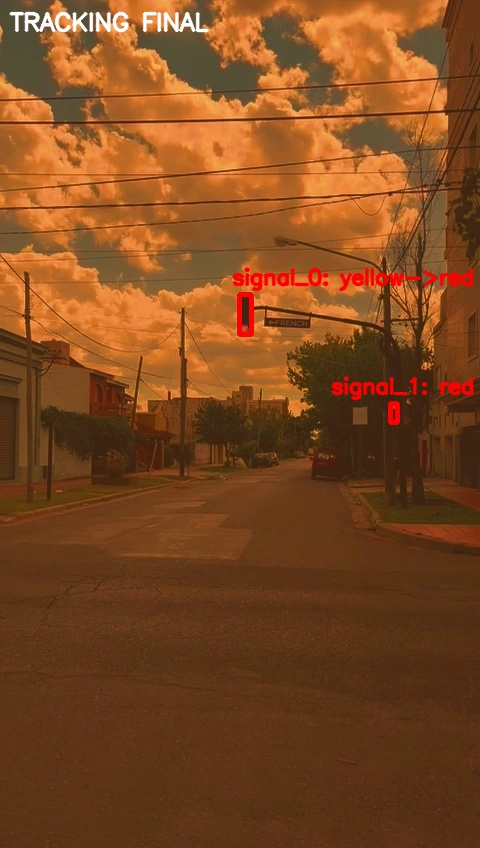
\includegraphics[width=0.7\textwidth]{yellow_espurio_v6_f1776.jpg}
    \caption[YELLOW espurio en Video~6, frame 1776.]{YELLOW espurio en el Video~6, \textit{frame} 1776, sobre \texttt{signal\_0}. El semáforo está en su fase de verde modificado (ámbar), pero el recognizer le asigna YELLOW; el \textit{tracker} lo corrige a RED por la regla asimétrica GREEN$\to$YELLOW$\to$RED. Es uno de los tres únicos \textit{frames} (de las 229 detecciones combinadas de las fases de falla en los Videos~5 y~6) donde se observa este fenómeno.}
    \label{fig:yellow_espurio}
\end{figure}

La Tabla~\ref{tab:csv_yellow_espurio} extrae las filas de los CSVs (\texttt{2\_recognition\_results.csv} y \texttt{3\_final\_results.csv}) en torno al \textit{frame} 1776 para que se pueda leer directamente la transición. Hasta el \textit{frame} 1775 el sistema venía estable en RED sobre \texttt{signal\_0}; en el 1776, primer \textit{frame} de la fase de verde modificado, el recognizer salta a YELLOW (con confianza alta del detector: \texttt{det\_vert} $= 0.97$), pero el \textit{tracker} lo rechaza. En los \textit{frames} 1777 y 1778 el recognizer ya pasa a BLACK ---el verde modificado dejó de ser una clase dominante para la red--- y el \textit{tracker} sigue sosteniendo RED por histéresis. Vale notar también que \texttt{signal\_1} (semáforo secundario) recién empieza a detectarse en el \textit{frame} 1776 y se comporta de forma estable en RED.

\begin{table}[H]
\centering
\small
\begin{tabular}{|c|c|c|c|c|c|}
\hline
\textbf{Frame} & \textbf{signal\_id} & \texttt{det\_vert} & \texttt{pred\_color} & \texttt{final\_color} & \texttt{tracker\_modified} \\
\hline
1774 & signal\_0 & 0.98 & red    & red & False \\
1775 & signal\_0 & 0.99 & red    & red & False \\
\hline
\textbf{1776} & \textbf{signal\_0} & \textbf{0.97} & \textbf{yellow} & \textbf{red} & \textbf{True} \\
1776 & signal\_1 & 0.60 & red    & red & False \\
\hline
1777 & signal\_0 & 0.96 & black  & red & True \\
1777 & signal\_1 & 0.59 & red    & red & False \\
1778 & signal\_0 & 0.96 & black  & red & True \\
\hline
\end{tabular}
\caption{Fragmento de los CSVs de salida del Video~6 en torno al YELLOW espurio del \textit{frame} 1776 sobre \texttt{signal\_0}. La columna \texttt{det\_vert} es la probabilidad del detector para la clase ``vertical'' (de \texttt{1\_detection\_results.csv}), e indica que la red de detección estaba confiada de que era un semáforo; \texttt{pred\_color} es la salida del recognizer, \texttt{final\_color} la salida del \textit{tracker}. La fila resaltada es la activación de la regla asimétrica GREEN$\to$YELLOW$\to$RED.}
\label{tab:csv_yellow_espurio}
\end{table}

\subsubsection{Factibilidad del Escenario en Condiciones Reales}

Si bien la alteración del Video 6 se generó sintéticamente, vale la pena especular sobre si una condición de iluminación real podría producir un efecto análogo. El verde modificado del Video 6 ---ámbar saturado con luminosidad elevada--- no es una invención arbitraria: visualmente se parece bastante a lo que un semáforo verde puede aparentar bajo ciertas condiciones físicas concretas:

\begin{itemize}
    \item \textbf{Luz solar directa al amanecer o atardecer:} el sol bajo proyecta una iluminación cálida sobre la cara del semáforo. Si la cubierta protectora de la luz verde refleja parcialmente esa luz cálida, el resultado para la cámara puede ser cromáticamente parecido al Video 6.
    \item \textbf{Reflejos de superficies cercanas:} carteles iluminados, fachadas anaranjadas, o luces de freno de vehículos cercanos pueden sumar componentes cálidas a la apariencia del semáforo.
    \item \textbf{Cámaras con balance de blancos desplazado:} si el sistema de cámaras del vehículo compensa una escena globalmente fría desplazando el balance hacia cálidos, las luces verdes podrían registrarse con un tono distinto al esperado por el modelo.
    \item \textbf{Semáforos con LEDs degradados o cubiertas amarillentas:} unidades viejas con cubiertas plásticas que han envejecido pueden tener verdes notablemente más cálidos de lo normal.
\end{itemize}

No es difícil imaginar combinaciones de estas condiciones que se acerquen al punto que el test identificó como crítico. El test no demuestra que el escenario sea físicamente realizable con un par específico de condiciones, pero el gradiente de los seis videos sugiere que la frontera entre ``robusto'' y ``falla'' es lo suficientemente próxima a alteraciones cromáticamente plausibles como para que el escenario no se pueda descartar a priori.

\subsubsection{Implicancias Upstream para el Sistema Completo}

Más importante todavía es preguntarse \textbf{qué le pasaría al resto del vehículo} si el TLR efectivamente reportara este modo de falla durante operación real. El TLR es un componente \textit{upstream} del módulo de planificación de Apollo: lo que el TLR diga sobre el estado del semáforo entra como evidencia en las decisiones de detenerse, avanzar o ceder paso. Los tres escenarios posibles del modo de falla, en orden de gravedad creciente desde el punto de vista de la planificación:

\begin{enumerate}
    \item \textbf{El TLR reporta BLACK} (apagado/desconocido) cuando el semáforo real está en verde. La planificación recibe una entrada ambigua. Dependiendo de cómo Apollo conjugue esa señal con el resto del contexto (presencia de la línea de detención, ausencia de vehículos cruzados, comportamiento de otros agentes), puede degradar a un comportamiento conservador: detener el vehículo o reducir velocidad. Es una falla incómoda pero relativamente segura.

    \item \textbf{El TLR reporta RED} cuando el semáforo real está en verde. Acá la planificación tiene información explícita y errónea: el semáforo está en rojo. El vehículo se detiene cuando físicamente podía avanzar. Es una falla \textit{molesta} (interrumpe el flujo del tráfico, expone al vehículo a colisiones por detrás), pero sigue siendo del lado conservador en términos de seguridad inmediata.

    \item \textbf{El TLR reporta YELLOW (en algún \textit{frame} puntual) y el \textit{tracker} no filtra.} Este caso no se observó en la salida final del test: el recognizer sí produjo YELLOW en tres \textit{frames} (1816 del Video 5; 1776 y 1856 del Video 6), pero el \textit{tracker} corrigió los tres a RED por la regla de seguridad, así que el YELLOW nunca llegó al downstream. Si por algún motivo la regla del \textit{tracker} fallara o el contexto previo no fuera RED, este escenario sí podría manifestarse: la interpretación de un amarillo intermitente por parte de la planificación es ambigua y depende del contexto, y el peor caso sería que el vehículo intente acelerar para ``pasar el amarillo''.
\end{enumerate}

Notablemente, ningún escenario observado en el test produce el peor caso posible de seguridad (que el TLR reporte GREEN cuando el semáforo real está en rojo). La asimetría de la regla GREEN$\to$YELLOW$\to$RED, en conjunto con la naturaleza del modo de falla observado (BLACK/RED dominante, YELLOW espurio neutralizado por el \textit{tracker}, no GREEN espurio), sugieren que el sistema falla del lado conservador. Esto no quiere decir que el modo de falla sea aceptable ---un vehículo autónomo que se detiene en falso en cada atardecer cálido sería un producto inviable--- pero sí explica por qué el diseño del TLR resiste el adversario que el test logró construir.

\subsection{Interacción con el \textit{tracker}: Respuesta Parcial}
\label{subsec:respuesta_parcial_tracker}

La parte interesante del test es lo que el \textit{tracker} hizo durante la fase de falla. Comparando la salida cruda del recognizer (registrada \textit{frame} a \textit{frame}) con la salida final del \textit{tracker}, se observan dos clases de intervenciones cuantitativamente muy distintas.

\textbf{Histéresis BLACK$\to$RED, mecanismo dominante.} Cada vez que el recognizer reporta BLACK durante la fase de verde modificado, el \textit{tracker} lo reemplaza por RED en la salida final, porque el color previo conocido para ese \textit{signal\_id} era RED. Esto explica por qué la salida final no muestra los BLACKs que el recognizer sí está produciendo: el \textit{tracker} los está amortiguando uno a uno. Es el efecto más visible y consistente del \textit{tracker} en este test.

La Figura~\ref{fig:histeresis_black_red} ilustra este mecanismo sobre un \textit{frame} concreto del Video~6: a la izquierda, la salida cruda del recognizer (BLACK, porque la probabilidad máxima cae por debajo del umbral de \texttt{Prob2Color}); a la derecha, la salida final del \textit{tracker} (RED, sostenido a partir del último color conocido). El contraste hace visible una de las 134 correcciones combinadas que el \textit{tracker} aplicó en las fases de falla de los Videos~5 y~6.

\begin{figure}[H]
    \centering
    \begin{subfigure}[t]{0.48\textwidth}
        \centering
        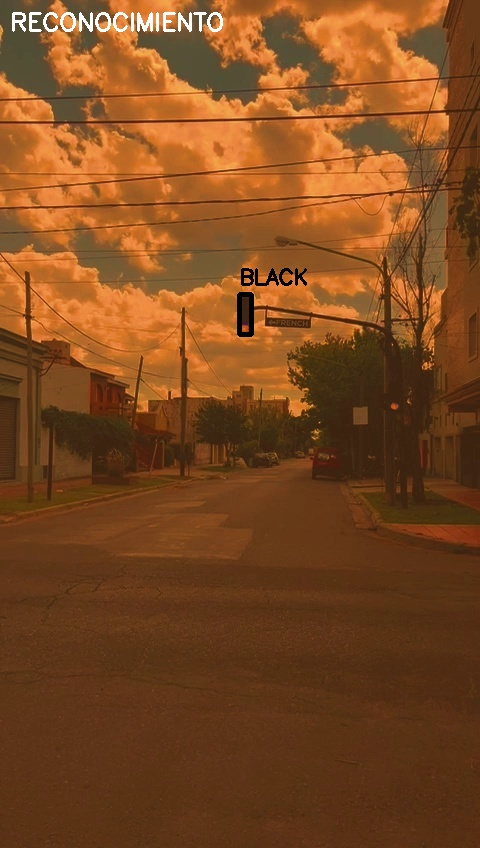
\includegraphics[width=\textwidth]{histeresis_v6_recognizer.jpg}
        \caption[Recognizer: BLACK.]{Salida cruda del recognizer: BLACK. La probabilidad máxima de la red queda por debajo de 0.5 y \texttt{Prob2Color} fuerza el color a apagado.}
        \label{fig:hist_rec}
    \end{subfigure}
    \hfill
    \begin{subfigure}[t]{0.48\textwidth}
        \centering
        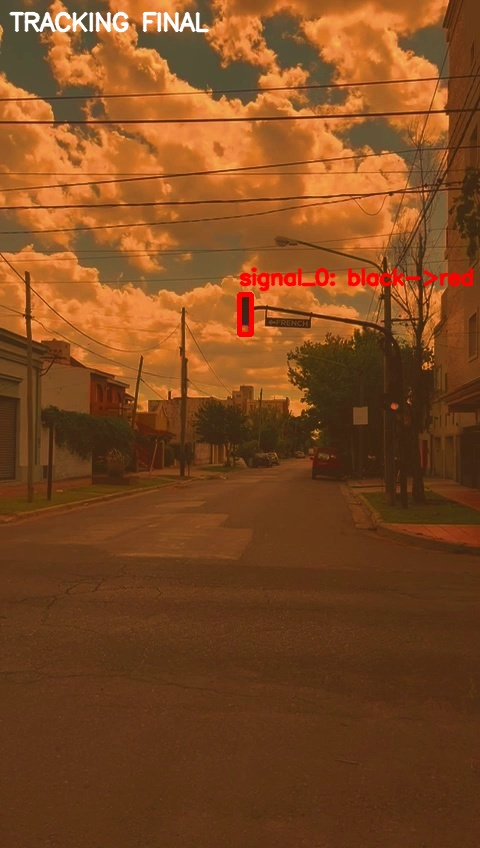
\includegraphics[width=\textwidth]{histeresis_v6_final.jpg}
        \caption[Tracker: RED (histéresis).]{Salida final del \textit{tracker}: RED. La histéresis para BLACK mantiene el color encendido del historial (RED de la fase rojo natural inmediatamente anterior).}
        \label{fig:hist_final}
    \end{subfigure}
    \caption[Histéresis BLACK$\to$RED del \textit{tracker} (Video~6).]{Histéresis BLACK$\to$RED del \textit{tracker} sobre un \textit{frame} del Video~6 en la fase de verde modificado. Es el mecanismo dominante de intervención del \textit{tracker} en el test: amortigua los BLACKs aislados del recognizer sosteniendo el último color encendido del historial. En total, 134 correcciones de este tipo se observan en las fases de falla combinadas de los Videos~5 y~6.}
    \label{fig:histeresis_black_red}
\end{figure}

La Tabla~\ref{tab:csv_histeresis} muestra una ventana del CSV del Video~6 (\textit{frames} 1823--1829, sobre \texttt{signal\_0}) que cubre los tres regímenes del mecanismo: corrección activa, agotamiento de la histéresis y reinicio. En 1823--1824 el \textit{tracker} corrige BLACK a RED como hace en la mayor parte de la fase. En 1825--1827, tres BLACK consecutivos del recognizer agotan la histéresis y el \textit{tracker} acepta BLACK como salida final (estos son los tres únicos BLACK que sobreviven en todo el Video~6). En el \textit{frame} 1828, el recognizer vuelve a reportar RED espontáneamente y el \textit{tracker} dispara la marca \texttt{(BLINK)} ---una de las cuatro únicas activaciones de \textit{blink status} en este video---, interpretando el patrón ``encendido $\to$ apagado prolongado $\to$ encendido'' como un parpadeo. En el \textit{frame} 1829 la oscilación BLACK/RED del recognizer reanuda y la histéresis vuelve a operar.

\begin{table}[H]
\centering
\small
\begin{tabular}{|c|c|c|c|c|c|}
\hline
\textbf{Frame} & \textbf{signal\_id} & \texttt{pred\_color} & \texttt{final\_color} & \texttt{blink\_status} & \texttt{tracker\_modified} \\
\hline
1823 & signal\_0 & black & red   &        & True  \\
1824 & signal\_0 & black & red   &        & True  \\
\hline
1825 & signal\_0 & black & \textbf{black} &        & False \\
1826 & signal\_0 & black & \textbf{black} &        & False \\
1827 & signal\_0 & black & \textbf{black} &        & False \\
\hline
1828 & signal\_0 & red   & red   & \textbf{(BLINK)} & False \\
1829 & signal\_0 & black & red   &        & True  \\
\hline
\end{tabular}
\caption{Fragmento del CSV de salida del Video~6 (\texttt{3\_final\_results.csv}) sobre \texttt{signal\_0} en la fase de verde modificado. Las tres secciones del cuadro muestran, en orden: la histéresis funcionando (BLACK corregido a RED), la histéresis agotada (tres BLACK consecutivos aceptados como final), y la activación de \texttt{(BLINK)} cuando el recognizer vuelve a reportar RED después del apagado sostenido.}
\label{tab:csv_histeresis}
\end{table}

\textbf{Corrección YELLOW$\to$RED, mecanismo minoritario.} En tres \textit{frames} puntuales repartidos entre los dos videos fallidos ---el \textit{frame} 1816 del Video 5, y los \textit{frames} 1776 (primer \textit{frame} de la fase, justo en la transición desde el rojo natural) y 1856 (cerca del final de la fase) del Video 6, los tres sobre \texttt{signal\_0}--- el recognizer reporta YELLOW. En las tres ocasiones el \textit{tracker} corrige el resultado a RED por la regla de seguridad asimétrica (YELLOW después de RED se rechaza). Este es el escenario que la regla está diseñada para filtrar, y los datos muestran que efectivamente actúa cuando aparece la oportunidad.

\subsubsection{El hallazgo es informativo pero estadísticamente débil}

El segundo mecanismo activa la pregunta que se había dejado abierta en versiones anteriores de este análisis: ¿la regla GREEN$\to$YELLOW$\to$RED actuó en este test? La respuesta es \textbf{sí, pero con una frecuencia muy baja}: tres detecciones en total (una en el Video 5, dos en el Video 6) sobre las $\sim$229 detecciones que el recognizer produjo en las fases de falla de los dos videos. El comportamiento dominante de esas fases es BLACK/RED, no YELLOW corregido a RED.

Esto deja la lectura en un estado intermedio, no concluyente:

\begin{itemize}
    \item \textbf{Por un lado,} el test sí documentó un caso concreto donde la regla intercepta un error real del clasificador, no sólo un caso hipotético. Es información que el aislamiento del módulo hizo posible (sin acceso a las salidas crudas del recognizer no habríamos podido ver el YELLOW espurio).

    \item \textbf{Por otro,} el peso estadístico del fenómeno es marginal frente al modo de falla principal (BLACK/RED). Tratar la activación observada como evidencia de un rol estructural de la regla en este escenario sería sobreinterpretar la evidencia que produjo esta corrida del test.
\end{itemize}

\subsubsection{Hipótesis a contrastar y extensiones}

Lo observado abre dos hipótesis sobre la naturaleza del fenómeno, que el test actual no permite zanjar:

\begin{enumerate}
    \item \textbf{Caso aislado.} El YELLOW espurio es un artefacto de los bordes de la fase de verde modificado (transiciones bruscas, primer \textit{frame} del nuevo estado), y no se reproduce de manera sistemática dentro del cuerpo de la fase. La regla actúa pero su rol cuantitativo es marginal.

    \item \textbf{Punta del iceberg.} La frecuencia baja es consecuencia de haber probado solo dos configuraciones en el lado fallido del umbral, sobre un único video base. Con configuraciones intermedias del parámetro de tono (entre $-80$ y $-100$) o con escenas distintas, aparecerían más \textit{frames} con YELLOW espurio, y la regla pasaría a tener un rol cuantitativamente relevante en filtrar la falla.
\end{enumerate}

Distinguir entre ambas hipótesis es trabajo inmediato y queda enmarcado en el Capítulo~\ref{cap:conclusiones}: probar configuraciones intermedias del parámetro de tono y repetir el test con escenas distintas, para evaluar si el fenómeno depende del contenido específico de la imagen o es genérico de la alteración cromática. El enfoque cambia ligeramente respecto a lo que se había planteado antes (cuando la pregunta era ``¿se activó la regla?''): ahora la pregunta es ``¿los casos observados son representativos o anecdóticos?''. Pero las herramientas necesarias para responderlo son las mismas, y todas las extensiones que se habían planteado siguen siendo válidas con este nuevo enfoque.

\section{Lo Aprendido sobre el Módulo TLR de Apollo}

\subsection{Decisiones de Diseño Extraídas del Código}

El proceso de análisis y aislamiento (Capítulos~\ref{cap:analisis_apollo}--\ref{cap:reimplementacion}) reconstruyó decisiones de diseño que no aparecen en la documentación oficial. Las más significativas:

\begin{itemize}
    \item \textbf{Ponderación 70/30 del algoritmo húngaro} entre proximidad espacial y confianza de detección: Apollo confía más en la geometría del HD-Map que en el \textit{score} de la red. Esto explica por qué detecciones cercanas con \textit{score} moderado pueden ganarle a detecciones lejanas con \textit{score} alto.

    \item \textbf{Ventana temporal de 1.5\,s en el \textit{tracker}, con histéresis y \textit{reset}.} El sistema valida transiciones dentro de esa ventana y resetea el historial cuando se pierde de vista al semáforo por más tiempo, lo que le permite recuperarse rápido de oclusiones largas sin perder reactividad en operación normal.

    \item \textbf{\textit{Blink detection} restringida al verde, con umbral de 0.55\,s.} Apollo solo marca \textit{blink} cuando el patrón ocurre sobre verde (típicamente, flechas verdes intermitentes que habilitan giros). Rojo y amarillo no producen \textit{blink flag}.

    \item \textbf{Asimetría de la regla GREEN$\to$YELLOW$\to$RED.} La regla en sí está documentada \cite{apollo_tlr_docs}, pero lo que el análisis aportó es el conjunto de detalles que la rodean en la implementación: en qué archivo vive, cómo se conjuga con la ventana temporal, qué pasa cuando se combina con BLACK. El test del Capítulo~\ref{cap:diseno_tests} le da una caracterización empírica a su alcance: cuál clase de fallas filtra y cuál no.
\end{itemize}

\subsection{Funcionalidad Diseñada pero No Efectiva}

El \texttt{semantic\_id} es el caso más llamativo. El código tiene infraestructura para agrupar semáforos del mismo cruce y aplicarles \textit{voting} ---es decir, corregir clasificaciones individuales a partir de la mayoría del grupo---, pero el \texttt{semantic\_id} está hardcodeado a 0 en \texttt{traffic\_light\_region\_proposal\_component.cc:335}, lo que reduce el \textit{voting} a una operación trivial sobre grupos de un solo elemento. La consecuencia práctica: no hay corrección por consistencia entre semáforos del mismo cruce.

Detectar esta brecha entre diseño e implementación habría sido difícil para alguien que solo usa Apollo como caja negra. El aislamiento por reconstrucción la hizo evidente porque obligó a recorrer línea por línea las cuatro carpetas del TLR durante el análisis.

\section{Lo Aprendido sobre la Metodología}

\subsection{Aislamiento por Reconstrucción vs.\ Recorte}

Las dos aproximaciones que se intentaron tuvieron resultados muy distintos. El detalle cuantitativo del intento de recorte está en el Apéndice~\ref{apendice:recorte_fallido}; en términos cualitativos:

\begin{itemize}
    \item Recortar el código original implicaba arrastrar más de 169\,000 líneas de infraestructura no funcional para que el TLR ejecutara, levantar CyberRT, dominar Bazel y mantener un \textit{stack} de GPU específico. El \textit{setup} estimado superaba uno o dos meses, sin garantías de cerrar.
    \item Aislar por reconstrucción produjo, sobre la base del análisis del código original, un módulo equivalente de $\sim$1\,900 líneas Python con dos dependencias (PyTorch, NumPy), ejecutable en minutos, modificable en tiempo real, instrumentable con \textit{prints} y \textit{breakpoints}.
\end{itemize}

La lección no es que reconstruir sea \textit{siempre} mejor que recortar. Es que, cuando el sistema legado tiene un acoplamiento profundo con su infraestructura (mensajería propia, \textit{build system} pesado, dependencias de hardware específicas), recortar puede no ser realmente más barato que reconstruir, aunque parezca el camino más corto.

\subsection{Valor del Conocimiento Interno para Testing}

El test del Capítulo~\ref{cap:diseno_tests} habría sido imposible de \textit{interpretar} sin el conocimiento interno acumulado durante el aislamiento. Un observador externo, viendo la tabla de fases del Video 6, vería un comportamiento difícil de explicar: el último tramo del ciclo (cuando el semáforo vuelve a verde) reporta RED y BLACK en la salida final, sin GREEN; y la salida cruda del recognizer agrega un par de YELLOW puntuales que no aparecen en el resultado del sistema. Con el conocimiento del recognizer (cuatro clases de salida), de \texttt{Prob2Color} (umbral 0.5 que fuerza BLACK por debajo), y del \textit{tracker} (regla asimétrica, histéresis), la misma tabla cuenta una historia coherente: el clasificador no reconoce el verde modificado y oscila entre BLACK y RED, el \textit{tracker} amortigua los BLACK por histéresis y corrige los pocos YELLOW espurios por la regla de seguridad.

Esto valida la hipótesis central del trabajo: para sistemas de \textit{machine learning} sin especificación formal, el testing efectivo necesita conocimiento interno; el conocimiento interno no se obtiene sin acceso al código; el acceso al código sin la posibilidad de ejecutarlo y modificarlo no alcanza. El aislamiento es lo que cierra esa cadena.

\subsection{Limitación Metodológica: Equivalencia por Construcción}

La equivalencia funcional entre el módulo aislado y el TLR de Apollo no se validó empíricamente: no se ejecutó Apollo sobre las mismas entradas para comparar salidas, porque el costo de hacerlo es desproporcionado al objetivo. La equivalencia se afirma bajo los doce supuestos explícitos enumerados en la sección~\ref{sec:supuestos_equivalencia} del Capítulo~\ref{cap:reimplementacion}. Los hallazgos del test deben leerse condicionalmente: ``si esos supuestos se cumplen, entonces el comportamiento observado en el módulo aislado es también el de Apollo''.

Es una limitación honesta del enfoque, no un defecto de ejecución. Un trabajo futuro que pueda invertir el costo de configurar Apollo podría hacer la comparación A/B y reducir el espacio de supuestos.

\section{Síntesis}

En conjunto, los tres planos de aprendizajes (clasificador, TLR de Apollo, metodología) refuerzan la idea con la que se abrió el trabajo. La efectividad del testing sobre un sistema de \textit{machine learning} embebido en una infraestructura compleja no depende solamente del esfuerzo invertido en correrlo: depende, sobre todo, de poder verlo desde adentro. Aislar el módulo fue lo que permitió diseñar un test específico, ejecutarlo, observar lo que pasaba en cada etapa, y construir una explicación coherente sobre el clasificador (que tolera alteraciones amplias del verde y falla puntualmente con una combinación específica de tono, luminosidad y saturación), sobre el \textit{tracker} (cuya regla asimétrica se activó en algunos \textit{frames} aislados pero con una frecuencia lo suficientemente baja como para que el rol estructural de esa activación tenga que ser corroborado en una corrida más densa), y sobre el diseño del TLR de Apollo (que decidió, hace tiempo, qué clase de fallas quería filtrar y bajo qué reglas).

\chapter{Conclusiones y Trabajo Futuro}
\label{cap:conclusiones}

\section{Conclusiones}

\subsection{Sobre la Metodología}

\textbf{Aislar fue más viable que recortar.} Para sistemas \textit{legacy} complejos como Apollo, intentar recortar un módulo del sistema completo no fue una opción realista: las 4\,800 líneas de C++ del TLR vienen acompañadas de aproximadamente 169\,000 líneas de infraestructura compartida (CyberRT, \textit{perception common}, \textit{modules common}, \textit{map module}), un sistema de \textit{build} pesado (Bazel), un entorno de despliegue específico (Docker + CUDA + GPU NVIDIA dedicada) y configuraciones extensas. El esfuerzo de \textit{setup}, sin garantías de cerrar, superaba uno o dos meses. El aislamiento por reconstrucción ---tomar el código original como especificación y reescribirlo en un entorno simple--- entregó el mismo módulo funcional en una fracción del costo, instrumentable con \textit{prints} y \textit{breakpoints}, sin dependencias de hardware específicas.

\textbf{El aislamiento por reconstrucción fuerza comprensión profunda.} El proceso de leer línea por línea las cuatro carpetas del TLR para reescribirlas obligó a extraer parámetros, reglas de negocio, casos especiales y decisiones de diseño que no aparecen en la documentación oficial. La elección de Python como lenguaje de destino fue por comodidad de prototipado, no por una propiedad esencial del enfoque; lo importante no fue el lenguaje, sino que el módulo terminara extraído de su entorno y bajo control directo.

\textbf{El intento de recorte no fue tiempo perdido.} Aunque la primera aproximación no produjo un módulo ejecutable, sí produjo el conocimiento conceptual del pipeline (etapas, dependencias, parámetros a alto nivel) que después alimentó tanto el análisis del Capítulo~\ref{cap:analisis_apollo} como la formulación del test del Capítulo~\ref{cap:diseno_tests}. Las preguntas que el test terminó respondiendo (¿qué hace el recognizer fuera de su distribución? ¿qué rol cumple la regla GREEN$\to$YELLOW$\to$RED?) nacieron durante esa fase fallida.

\subsection{Sobre el Testing}

\textbf{El conocimiento interno habilita tests que la caja negra no puede formular.} El test del Capítulo~\ref{cap:diseno_tests} se diseñó a partir de objetos internos del módulo: las cuatro clases del recognizer, la regla \texttt{Prob2Color} con su umbral 0.5, la asimetría de la regla GREEN$\to$YELLOW$\to$RED. Sin conocer la estructura interna del clasificador, un test de caja negra podría haber probado variaciones de iluminación, pero le habría costado mucho más \textit{interpretar} los resultados: por qué BLACK aparece, por qué oscila con RED, y por qué los pocos YELLOW que el recognizer sí produce en la fase de falla nunca llegan a la salida final del sistema.

\textbf{El testing iterativo se beneficia del aislamiento.} Cada variante del test ---un video nuevo, una configuración nueva de tono/luminosidad/saturación--- se procesó con una llamada Python sobre el módulo aislado, en segundos. Iterar a esa velocidad sobre Apollo habría requerido recompilar y redesplegar entre cada cambio. La velocidad de iteración no es solo cuestión de productividad: es lo que permite reformular hipótesis y refinar el test hasta encontrar el adversario.

\textbf{El test produjo dos clases de resultados.} El primero, concreto: el clasificador del módulo es robusto a alteraciones cromáticas moderadas del verde y empieza a fallar a partir de la configuración del Video 5 (Tono $-100$ + luminosidad $+10$ + saturación $+20$); la falla se intensifica en el Video 6 (Tono $-110$). El umbral de falla queda ubicado entre tonos $-80$ y $-100$. El segundo, parcial: comparando la salida cruda del recognizer con la salida final del \textit{tracker}, se observan dos clases de intervención del \textit{tracker} durante la fase de falla ---histéresis BLACK$\to$RED dominante (134 correcciones combinadas en los Videos 5 y 6), y corrección YELLOW$\to$RED puntual por la regla asimétrica (3 correcciones en total: una en el Video 5 sobre el \textit{frame} 1816, dos en el Video 6 sobre los \textit{frames} 1776 y 1856)---, pero la frecuencia de la segunda es lo suficientemente baja como para que el hallazgo abra una pregunta cuantitativa más que cerrarla. La pregunta deja de ser ``¿se activó la regla?'' (sí, en tres \textit{frames}) y pasa a ser ``¿los casos observados son representativos del modo de falla o artefactos puntuales?'' (Sección~\ref{sec:trabajo_futuro_inmediato}).

\subsection{Sobre el Sistema Apollo}

\textbf{Decisiones de diseño no documentadas.} El análisis reveló aspectos que no aparecen en la documentación oficial: la ponderación 70/30 entre proximidad espacial y confianza del algoritmo húngaro, la ventana temporal de 1.5\,s del \textit{tracker} con histéresis, y la restricción del \textit{blink detection} al color verde con umbral de 0.55\,s. La regla GREEN$\to$YELLOW$\to$RED sí está documentada \cite{apollo_tlr_docs}; lo que el análisis aportó es el conjunto completo de reglas que la rodean en la implementación.

\textbf{Funcionalidad diseñada pero no efectiva.} El \texttt{semantic\_id} está hardcodeado a 0 en \texttt{traffic\_light\_region\_proposal\_component.cc:335}, lo que reduce el \textit{voting} entre semáforos del mismo cruce a una operación trivial sobre grupos de un solo elemento. La funcionalidad existe en el código pero no aporta nada en la práctica.

\textbf{El TLR falla del lado conservador.} El modo de falla observado en el test no produce el peor caso posible de seguridad (que el TLR reporte GREEN cuando el semáforo real está en rojo). Las salidas erróneas son BLACK o RED, que conducen a comportamientos conservadores de la planificación (detenerse, esperar). La asimetría de la regla del \textit{tracker} contribuye a este sesgo: si el clasificador alguna vez se confunde hacia ``más permisivo'' (YELLOW después de RED), la regla lo corrige hacia ``más restrictivo''.

\section{Contribuciones}

\begin{enumerate}
    \item \textbf{Metodología:} formulación del aislamiento por reconstrucción como herramienta para habilitar testing dirigido sobre componentes de \textit{machine learning} embebidos en sistemas legacy complejos, con la primera aproximación de recorte documentada como contraste.

    \item \textbf{Análisis funcional del TLR de Apollo:} documentación de parámetros, reglas y decisiones de diseño no explicitadas en la documentación oficial (ponderación 70/30 del algoritmo húngaro, ventana temporal de 1.5\,s con histéresis, \textit{blink detection} restringido al verde con umbral de 0.55\,s, \texttt{semantic\_id} hardcodeado a 0).

    \item \textbf{Módulo aislado:} paquete Python equivalente al TLR de Apollo a nivel funcional, ejecutable sin la infraestructura del vehículo, con API simple y código modificable.

    \item \textbf{Definición de supuestos de equivalencia:} doce supuestos explícitos bajo los cuales el módulo aislado se considera fiel al original, dejando claro que la equivalencia es por construcción y no empírica.

    \item \textbf{Test de transición verde$\to$amarillo:} caracterización del límite de robustez del clasificador del TLR, con identificación del umbral de falla (entre tono $-80$ y $-100$ con cambios acompañantes de luminosidad y saturación), discusión de la factibilidad física del escenario y análisis de las consecuencias \textit{upstream} para el sistema completo.

    \item \textbf{Validación de la hipótesis:} demostración concreta de que el conocimiento interno del sistema permite diseñar y, sobre todo, \textit{interpretar} tests; sin ese conocimiento, los resultados del experimento serían ruido en lugar de un fenómeno explicable.
\end{enumerate}

\section{Limitaciones}

\subsection{Del Test}

\textbf{Adversario sintético.} La alteración de color se realiza digitalmente con un editor de video. El Capítulo~\ref{cap:resultados} discute en qué condiciones físicas reales (luz solar baja al amanecer/atardecer, reflejos cálidos, cámaras con balance de blancos desplazado, semáforos con LEDs envejecidos) podría producirse un efecto cromáticamente parecido, pero el test no demuestra que esas condiciones específicas reproduzcan exactamente el modo de falla.

\textbf{Cobertura limitada.} Solo se exploró una dirección de alteración (verde hacia tonos cálidos). Otras fronteras del clasificador (amarillo$\to$rojo, rojo$\to$apagado, comportamiento bajo oclusiones que activen el \textit{reset} del \textit{tracker}) no fueron testeadas sistemáticamente.

\textbf{Dos configuraciones críticas sobre una sola escena.} La corrida procesó los 1\,859 \textit{frames} completos del video sobre dos configuraciones del lado fallido del umbral (Video 5: Tono $-100$ + luminosidad $+10$ + saturación $+20$; Video 6: Tono $-110$ + luminosidad $+10$ + saturación $+20$) y un único video base. Las tres activaciones observadas de la regla GREEN$\to$YELLOW$\to$RED son pocas como para afirmar si son representativas del modo de falla o si son artefactos puntuales que se comportarían distinto bajo otras condiciones. Cerrar esa duda requiere probar configuraciones intermedias del parámetro de tono y repetir el test sobre escenas distintas.

\textbf{Cobertura limitada de configuraciones.} Aunque el video se procesó a 30\,fps completos (1\,859 \textit{frames}) sobre las seis configuraciones, solo dos configuraciones quedaron del lado fallido del umbral (Videos 5 y 6), sin barrer valores intermedios de tono entre $-80$ y $-100$, ni explorar combinaciones distintas de luminosidad y saturación cerca del umbral. Refinar el punto exacto donde el clasificador empieza a fallar requiere ese barrido.

\subsection{Del Módulo Aislado}

\textbf{Interfaz simplificada con \textit{projection boxes}.} El módulo aislado no reproduce la generación dinámica de \textit{projection boxes} desde el HD-Map: las recibe pre-calculadas en un archivo, con \texttt{signal\_id} estable. Esto limita ciertos escenarios de testing que dependen de errores de pose o de calibración dinámica de cámara.

\textbf{Equivalencia por construcción.} La equivalencia funcional con Apollo no se validó empíricamente comparando salidas sobre las mismas entradas. La equivalencia se afirma por construcción, bajo los doce supuestos explícitos enumerados en la Sección~\ref{sec:supuestos_equivalencia} del Capítulo~\ref{cap:reimplementacion}. Todo hallazgo del trabajo es condicional a que esos supuestos se cumplan.

\subsection{De la Generalización}

Los hallazgos son específicos del módulo TLR de Apollo y del test concreto que se diseñó. No podemos afirmar a priori que la metodología produzca resultados similares en otros módulos de Apollo o en otros sistemas \textit{legacy}, aunque el patrón ---intento de recorte fallido, análisis del código, aislamiento por reconstrucción, testing con conocimiento interno--- parece transferible al menos en términos conceptuales.

\section{Trabajo Futuro}

\subsection{Extensiones Inmediatas}
\label{sec:trabajo_futuro_inmediato}

\begin{itemize}
    \item \textbf{Resolver si la activación de la regla del \textit{tracker} es estructural o puntual.} La corrida sobre los dos videos fallidos detectó tres \textit{frames} donde el recognizer reportó YELLOW espurio (1816 en el Video 5; 1776 y 1856 en el Video 6) y el \textit{tracker} los corrigió a RED. La frecuencia (3 sobre $\sim$229 detecciones combinadas de las fases de falla) es lo suficientemente baja como para que el hallazgo sea informativo y no concluyente. Probar configuraciones intermedias del parámetro de tono entre $-80$ y $-100$ y repetir el test sobre escenas distintas permitiría determinar si el YELLOW espurio aparece sistemáticamente en la fase de falla o si es un fenómeno puntual.

    \item \textbf{Refinar el umbral de falla.} Generar videos con tonos intermedios entre $-80$ y $-100$ (por ejemplo $-85$, $-90$, $-95$) para acotar mejor la frontera entre robustez y falla. Repetir variando luminosidad y saturación por separado para entender si el modo de falla depende del tono solo o requiere la combinación de los tres parámetros.

    \item \textbf{Explorar otras fronteras del recognizer.} Aplicar la misma metodología a otros colores: alterar el rojo del semáforo y observar si el recognizer lo confunde con amarillo, alterar el amarillo y ver si lo confunde con verde o con rojo. Cada frontera caracterizada agrega información concreta sobre la topología del espacio de \textit{features} del modelo.

    \item \textbf{Activar deliberadamente la regla de seguridad.} Diseñar un experimento donde el recognizer reporte YELLOW después de RED con certeza (por ejemplo, intercalando \textit{frames} con un semáforo amarillo real entre \textit{frames} con un semáforo rojo real, sobre videos con condiciones controladas). Esto permitiría observar y caracterizar la regla GREEN$\to$YELLOW$\to$RED actuando de forma explícita.
\end{itemize}

\subsection{Extensiones a Mediano Plazo}

\begin{itemize}
    \item \textbf{Validar empíricamente la equivalencia con Apollo.} Configurar Apollo (asumiendo el costo de \textit{setup} del Apéndice~\ref{apendice:recorte_fallido}) y correr ambos sistemas sobre el mismo conjunto de entradas para comparar salidas. Reduciría el espacio de supuestos del Capítulo~\ref{cap:reimplementacion} de doce a un subconjunto más pequeño.

    \item \textbf{Aplicar la metodología a otros módulos de Apollo.} Detección de peatones, detección de carriles, planificación local. Testear si el patrón ``recorte fallido $\to$ aislamiento por reconstrucción $\to$ testing con conocimiento interno'' se generaliza, o si depende de propiedades específicas del TLR (espacio de salida pequeño, dependencia clara de cámaras).

    \item \textbf{Estudiar el impacto del \texttt{semantic\_id} si se implementara.} Modificar el módulo aislado para usar \texttt{semantic\_id} real y \textit{voting} entre semáforos del mismo cruce, y evaluar cuánto mejora la robustez en escenarios con contradicciones entre detecciones individuales.
\end{itemize}

\subsection{Direcciones de Investigación}

\begin{itemize}
    \item \textbf{Formalización del aislamiento por reconstrucción.} Caracterizar qué propiedades de un módulo lo hacen apto para este enfoque (acoplamiento estructural vs.\ acoplamiento informacional, dependencias de hardware, tamaño relativo al sistema), y formular criterios para decidir cuándo conviene aislar versus invertir en levantar el sistema completo.

    \item \textbf{Métricas de equivalencia funcional.} Desarrollar formas de validar la equivalencia entre dos implementaciones de un módulo de \textit{machine learning} más allá de la comparación por construcción. Esto incluiría métricas de equivalencia distribucional (¿qué tan parecidas son las distribuciones de salida sobre la misma distribución de entradas?) y métricas de equivalencia comportamental sobre escenarios sintéticos.

    \item \textbf{Derivación sistemática de tests a partir de código.} Explorar herramientas que extraigan automáticamente parámetros críticos, fronteras de decisión y reglas asimétricas del código de un módulo, y propongan casos de test específicos a partir de ese análisis. El test del Capítulo~\ref{cap:diseno_tests} se diseñó a mano; una iteración del enfoque podría usar ese mismo proceso de manera sistemática.
\end{itemize}

\section{Reflexión Final}

Para testear efectivamente un sistema de \textit{machine learning} embebido en una infraestructura compleja, no alcanza con ejercitarlo desde afuera. La efectividad del testing depende de poder ver el sistema desde adentro: conocer sus parámetros, sus reglas, sus casos especiales, sus decisiones asimétricas. Ese conocimiento, sobre un sistema como Apollo, no se obtiene leyendo la documentación. Se obtiene leyendo el código. Y leer el código de manera útil ---hasta el nivel de poder ejercitarlo, instrumentarlo y reformularlo--- requiere extraerlo del entorno donde vive.

Este trabajo intentó dos caminos para conseguir esa extracción. El primero ---recortar el código original--- no cerró por el peso de la infraestructura asociada. El segundo ---aislar por reconstrucción--- sí cerró, y permitió diseñar un test que reveló a la vez algo sobre el clasificador (su robustez y su modo de falla concreto), algo sobre el \textit{tracker} (las dos explicaciones plausibles, ambas informativas) y algo sobre el diseño del TLR de Apollo (que sus reglas de seguridad están pensadas para filtrar el peor caso, aunque el experimento expuso bordes donde sus garantías son menos claras de lo que sugiere la documentación).

La contribución principal de este trabajo no es el módulo aislado en sí: es la demostración de que la cadena \textit{recorte fallido $\to$ aislamiento $\to$ testing dirigido} produce, sobre un sistema concreto, resultados que ni el testing de caja negra ni el análisis estático aislado habrían producido. Las preguntas sembradas durante el recorte se respondieron durante el aislamiento; las que quedaron abiertas tienen, ahora, un camino claro para cerrarse.

% ******************************************************** %
% ~~~~~~~~            BIBLIOGRAFÍA               ~~~~~~~~~ %
% ******************************************************** %

\bibliographystyle{plain}
\bibliography{bibliography/referencias}

% ******************************************************** %
% ~~~~~~~~              APÉNDICES                ~~~~~~~~~ %
% ******************************************************** %

\appendix
\chapter{Guía de Uso del Sistema}
\label{apendice:guia_uso}

Este apéndice proporciona instrucciones detalladas para instalar, configurar y utilizar el módulo aislado de detección de semáforos.

\section{Requisitos del Sistema}

\subsection{Hardware Recomendado}

\begin{table}[H]
\centering
\begin{tabular}{|l|l|}
\hline
\textbf{Componente} & \textbf{Especificación} \\
\hline
CPU & Intel i5/i7 o AMD equivalente (multi-core) \\
RAM & Mínimo 8 GB, recomendado 16 GB \\
GPU & NVIDIA con soporte CUDA (opcional pero recomendado) \\
Almacenamiento & 5 GB libres \\
\hline
\end{tabular}
\caption{Requisitos de hardware}
\end{table}

\subsection{Software Requerido}

\begin{itemize}
    \item Python 3.7 o superior
    \item CUDA Toolkit (opcional, si se usa GPU)
    \item Sistema operativo: Linux (Ubuntu 18.04+), macOS, o Windows 10+
\end{itemize}

\section{Instalación}

\subsection{Clonar el Repositorio}

\begin{codesnippet}
\begin{verbatim}
git clone [URL_DEL_REPOSITORIO]
cd TrafficLightDetection
\end{verbatim}
\end{codesnippet}

\subsection{Crear Entorno Virtual (Recomendado)}

\begin{codesnippet}
\begin{verbatim}
# Crear entorno virtual
python3 -m venv venv

# Activar entorno
# En Linux/macOS:
source venv/bin/activate
# En Windows:
venv\Scripts\activate
\end{verbatim}
\end{codesnippet}

\subsection{Instalar Dependencias}

\begin{codesnippet}
\begin{verbatim}
pip install -r requirements.txt
\end{verbatim}
\end{codesnippet}

Las principales dependencias incluyen:
\begin{itemize}
    \item PyTorch $\geq$ 1.8.0
    \item torchvision
    \item NumPy
    \item OpenCV (cv2)
    \item Matplotlib
\end{itemize}

\subsection{Verificar Instalación}

\begin{codesnippet}
\begin{verbatim}
# Verificar PyTorch
python -c "import torch; print(torch.__version__)"

# Verificar CUDA (si aplica)
python -c "import torch; print(torch.cuda.is_available())"
\end{verbatim}
\end{codesnippet}

\section{Uso Básico}

\subsection{API Principal}

El punto de entrada principal es la función \texttt{load\_pipeline()}:

\begin{codesnippet}
\begin{verbatim}
from tlr.pipeline import load_pipeline
import cv2

# Cargar pipeline
# Para GPU:
pipeline = load_pipeline('cuda:0')
# Para CPU:
# pipeline = load_pipeline('cpu')

# Cargar imagen
image = cv2.imread('path/to/image.jpg')

# Definir projection boxes
# Formato: [x1, y1, x2, y2] para cada ROI
projection_boxes = [
    [100, 50, 150, 120],  # box 1
    [500, 80, 550, 150],  # box 2
]

# Ejecutar detección
result = pipeline(image, projection_boxes)

# Resultado contiene:
# - result['bboxes']: coordenadas de semáforos detectados
# - result['colors']: estado de cada semáforo
# - result['scores']: confianza de cada detección
\end{verbatim}
\end{codesnippet}

\subsection{Procesamiento de Video}

\begin{codesnippet}
\begin{verbatim}
import cv2
from tlr.pipeline import load_pipeline

# Cargar pipeline
pipeline = load_pipeline('cuda:0')

# Abrir video
cap = cv2.VideoCapture('video.mp4')
frame_count = 0

while cap.isOpened():
    ret, frame = cap.read()
    if not ret:
        break

    # Procesar frame
    # (projection_boxes debería venir de HD-map o archivo)
    result = pipeline(frame, projection_boxes)

    # Visualizar resultados
    for bbox, color, score in zip(result['bboxes'],
                                   result['colors'],
                                   result['scores']):
        x1, y1, x2, y2 = bbox
        cv2.rectangle(frame, (x1, y1), (x2, y2), (0, 255, 0), 2)
        cv2.putText(frame, f'{color} ({score:.2f})',
                   (x1, y1-10), cv2.FONT_HERSHEY_SIMPLEX,
                   0.5, (0, 255, 0), 2)

    # Mostrar frame
    cv2.imshow('Traffic Light Detection', frame)
    if cv2.waitKey(1) & 0xFF == ord('q'):
        break

    frame_count += 1

cap.release()
cv2.destroyAllWindows()
\end{verbatim}
\end{codesnippet}

\section{Scripts Principales}

A continuación se describen los scripts principales utilizados para el flujo de trabajo del sistema.

\subsection{Extracción de Frames}

\begin{codesnippet}
\begin{verbatim}
python frames_extractor.py
\end{verbatim}
\end{codesnippet}

Extrae frames de un video para su posterior procesamiento. El video de entrada se selecciona directamente en el código del script, modificando la variable correspondiente al path del archivo de video.

\subsection{Selección de Projection Boxes}

\begin{codesnippet}
\begin{verbatim}
python select_projection_and_append.py
\end{verbatim}
\end{codesnippet}

Herramienta interactiva para seleccionar las projection boxes (ROIs donde se espera encontrar semáforos) manualmente usando el mouse. Las coordenadas seleccionadas se guardan en un archivo de texto para su uso posterior.

\subsection{Propagación de Projection Boxes}

\begin{codesnippet}
\begin{verbatim}
python propagate.py
\end{verbatim}
\end{codesnippet}

Propaga las projection boxes definidas en un frame a todos los frames extraídos del video. Útil cuando las projection boxes son válidas para toda la secuencia de frames.

\subsection{Ejecución del Pipeline}

\begin{codesnippet}
\begin{verbatim}
python run_pipeline.py
\end{verbatim}
\end{codesnippet}

Ejecuta el pipeline completo de detección de semáforos sobre los frames extraídos, utilizando las projection boxes definidas. Genera los resultados de detección y clasificación para cada frame.

\section{Estructura de Directorios del Proyecto}

\begin{verbatim}
TrafficLightDetection/
+-- src/
|   +-- tlr/
|       +-- pipeline.py           # Pipeline principal
|       +-- detector.py           # Detector de semaforos
|       +-- recognizer.py         # Clasificadores
|       +-- tracking.py           # Tracking temporal
|       +-- selector.py           # Asignacion hungara
|       +-- hungarian_optimizer.py
|       +-- utils.py              # Utilidades
|       +-- weights/              # Modelos pre-entrenados
|       +-- confs/                # Configuraciones
+-- inputTesis/                   # Videos de entrada
+-- docs/                         # Documentacion
|   +-- tesis/                    # Documentos de la tesis
|   +-- ...
+-- requirements.txt              # Dependencias
+-- README.md                     # Readme del proyecto
\end{verbatim}

\chapter{Intento Fallido: Recorte de Apollo}
\label{apendice:recorte_fallido}

Este apéndice documenta el primer enfoque que se intentó antes de decidir reimplementar desde cero: intentar recortar el módulo TLR del sistema Apollo completo.

\section{Estrategia Inicial}

La idea era aislar el módulo TLR del código completo de Apollo:

\begin{enumerate}
    \item Clonar el repositorio completo de Apollo
    \item Identificar el módulo de percepción de semáforos
    \item Eliminar progresivamente dependencias innecesarias
    \item Mantener solo el código esencial para TLR
\end{enumerate}

\section{Problemas Encontrados}

\subsection{Complejidad del Sistema}

\begin{itemize}
    \item \textbf{Tamaño del código:} Millones de líneas de código C++
    \item \textbf{Dependencias profundas:} El módulo TLR dependía de:
    \begin{itemize}
        \item CyberRT: Framework de mensajería propio de Apollo
        \item Librerías de utilidades internas
        \item Configuraciones específicas del ecosistema Apollo
    \end{itemize}
\end{itemize}

\subsection{Requisitos de Configuración}

Apollo requiere una configuración extensa:

\begin{table}[H]
\centering
\begin{tabular}{|l|l|}
\hline
\textbf{Componente} & \textbf{Requisito} \\
\hline
CPU & 8+ cores \\
RAM & 16 GB \\
GPU & NVIDIA RTX 20xx+ \\
OS & Ubuntu 18.04/20.04/22.04 \\
CUDA & 11.8 \\
Docker & $\geq$ 19.03 \\
Espacio disco & $\sim$50 GB \\
\hline
\end{tabular}
\caption{Requisitos de hardware/software de Apollo}
\end{table}

\subsection{Proceso de Compilación}

La compilación de Apollo involucra:
\begin{enumerate}
    \item Descargar imagen Docker ($\sim$15 GB)
    \item Configurar container con NVIDIA runtime
    \item Compilar todo el sistema (30+ minutos en hardware típico)
    \item Resolver dependencias de Bazel (sistema de build)
\end{enumerate}

\subsection{Errores Encontrados}

Durante los intentos de recorte, se encontraron múltiples errores:

\begin{itemize}
    \item Errores crípticos de Bazel al remover dependencias
    \item Conflictos de versiones entre librerías internas
    \item Problemas de linking al intentar compilar módulos aislados
    \item Errores de runtime por falta de configuraciones de CyberRT
\end{itemize}

\section{Tiempo Invertido}

Se invirtieron varias semanas intentando:
\begin{itemize}
    \item Configurar el ambiente de desarrollo
    \item Entender el sistema de build
    \item Identificar y remover dependencias
    \item Resolver errores de compilación
\end{itemize}

Sin lograr una versión ejecutable del módulo TLR aislado.

\section{Razones del Fracaso}

\begin{enumerate}
    \item \textbf{Acoplamiento estrecho:} El código de Apollo está diseñado para funcionar como un sistema integrado, no como módulos independientes

    \item \textbf{CyberRT como dependencia central:} El framework de mensajería está entrelazado con toda la lógica de negocio

    \item \textbf{Falta de documentación:} No hay guías para extraer módulos individuales

    \item \textbf{Complejidad del build:} Bazel hace difícil entender qué dependencias son realmente necesarias
\end{enumerate}

\section{Lección Aprendida}

Esta experiencia motivó el cambio de estrategia hacia la reimplementación. La lección principal fue:

\textbf{Para sistemas legacy complejos con alto acoplamiento, reimplementar un subsistema desde cero puede ser más viable que intentar extraerlo del sistema original.}

La reimplementación, aunque requiere más trabajo inicial de análisis, produce un artefacto mucho más manejable y comprensible.

\section{Valor del Intento Fallido}

Aunque el recorte no funcionó, el intento no fue tiempo perdido:

\begin{itemize}
    \item Reveló la complejidad real del sistema
    \item Motivó la búsqueda de alternativas
    \item Generó familiaridad inicial con el código de Apollo
    \item Informó las decisiones de diseño de la reimplementación
\end{itemize}

\end{document}
